% This is not necessarily in the format for a VUW thesis chapter.

% Finished March 22, 2013

\documentclass[a4paper]{report}

\usepackage{amssymb, amsmath}
\usepackage{tikz}
\usetikzlibrary{calc}

\usepackage{marvosym}


\title{Chapter 2: Mixed Slip Flow}
\author{Nat Lund}

\newcommand{\beff}{\ensuremath{b_{\mathrm{eff}}}}
\newcommand{\bhigh}{\ensuremath{b_{\mathrm{high}}}}
\newcommand{\blow}{\ensuremath{b_{\mathrm{low}}}}
\newcommand{\phislip}{\ensuremath{\phi_{\mathrm{slip}}}}
\newcommand{\phisol}{\ensuremath{\phi_{\mathrm{solid}}}}
\newcommand{\sigsol}{\ensuremath{\sigma_{\mathrm{solid}}}}
\newcommand{\gamsol}{\ensuremath{ \dot{\gamma}_{\mathrm{solid}} }} 

\newcommand{\sep}{\begin{equation*} \star \end{equation*}}

\begin{document}
\maketitle

\section{Mixed Slip Surfaces}

While the boundary condition in classical fluid mechanics is homogeneous (`no slip'), and we are satisfied that fluid slip can indeed occur on an atomically flat homgeneous surface, we now turn our attention to \emph{mixed-slip} surfaces.
That is, surfaces that are heterogeneous --- where the intrinsic slip length is different on different parts of the surface.

While there could in principle be an infinite variety of mixed-slip surfaces, only two broad classes are important.  This is because physical mixed-slip surfaces almost always feature a liquid-\emph{air} interface, along with the the more familiar liquid-solid interface.  And there are two canonical configurations: superhydrophobic, and nanobubbles.

\subsection{Superhydrophobic Surfaces}

Recall that when a droplet of water sits on a surface, a contact angle $\theta$ is defined:

\begin{center}
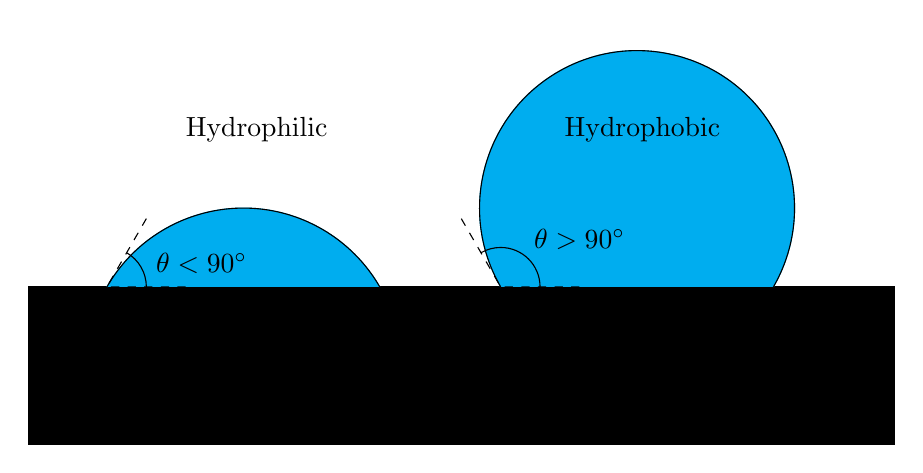
\begin{tikzpicture}
\filldraw (-1,0) rectangle +(11,-2); 

\filldraw[color=cyan] (0,0) arc (150:30:2);
\draw (0,0) arc (150:30:2);

\draw[dashed] (1,0) -- (0,0) -- (0.5,0.866);
\draw (0.5,0) arc (0:60:0.5);
\node at (0.5,0.3)[right] {$\theta < 90^{\circ}$};

\filldraw[color=cyan] (5,0) arc (210:-30:2);
\draw (5,0) arc (210:-30:2);

\draw[dashed] (6,0) -- (5,0) -- +(-0.5,0.866);
\draw (5.5,0) arc (0:120:0.5);
\node at (5.3,0.6)[right] {$\theta > 90^{\circ}$};

\node at (1.9,2) {Hydrophilic};
\node at (6.8,2) {Hydrophobic};

\end{tikzpicture}
\end{center}

Usually, a surface is defined as \emph{hydrophobic} when the contact angle is more than $90^{\circ}$.  This means that the water molecules are more attracted to each other than they are to the surface. (If $\theta < 90^{\circ}$, the surface is \emph{hydrophilic}.  If $\theta \sim 0^{\circ}$, then \emph{complete wetting} occurs: the water spreads out as far as it can.)

Tiny, micron or nanometer scale pillars can be constructed out of hydrophobic material.  A collection of theses hydrophobic nanopillars can be affixed to a suitable substrate, forming a `nanoforest'.  (Or, more practically, a nanoforest can be constructed, then chemically treated to become hydrophobic.)  If a water droplet is placed on top of the nanoforest, two curious things happen:  First, the droplet sits on the tops of the nanopillars, supported by surface tension.

\begin{center}
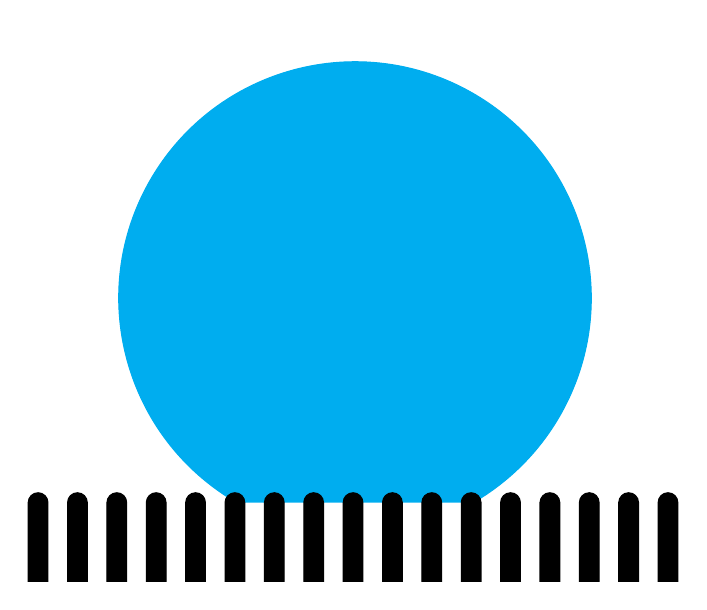
\begin{tikzpicture}

\filldraw[color=cyan] (3.15,1) arc (240:-60:3);

\foreach \x in {1,2,...,17}
{ \filldraw (\x/2,0) rectangle +(0.25,1) arc (0:180:0.125); }

\end{tikzpicture}
\end{center}

Second, the apparent contact angle is very large.  This second effect is caused by the fact that at the point where the contact line is located, the solid surface is at an angle to the plane of the nanoforest.

\begin{center}
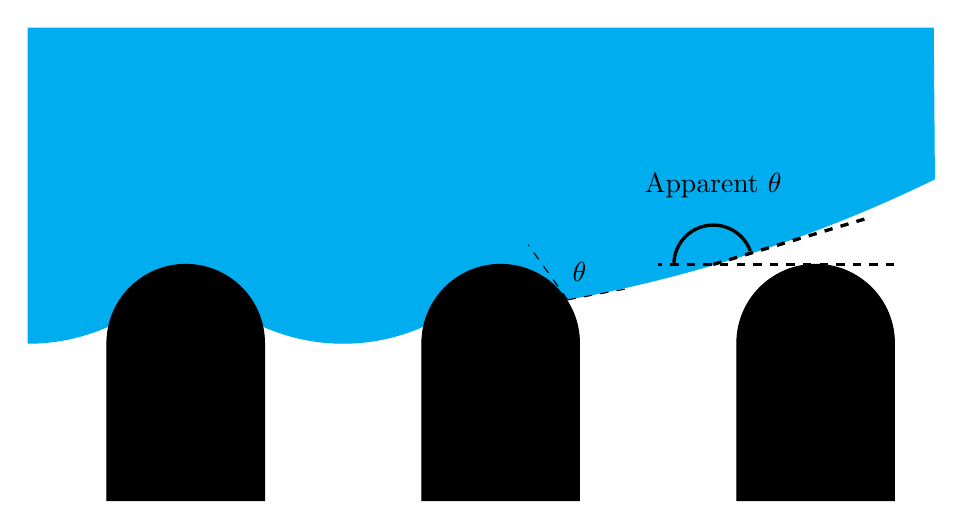
\begin{tikzpicture}

\filldraw[color=cyan] (10.5,6) -- (-1,6) -- (-1,2) arc (270:300:2.5)  -- +(1.5,0) arc (240:300:2.5) -- 
(5.75,2.54)  arc (-80:-64:18);

\foreach \x in {0,1,2}
\filldraw (\x*4,0) rectangle +(2,2) arc (0:180:1);

\draw[dashed] (5.85,2.55) -- +(-0.5,0.7);
\draw[dashed] (5.85,2.55) -- +(0.8,0.15);
\node at (6,2.9) {$\theta$};

\draw[very thick, dashed] (10, 3) -- +(-3,0);
\draw[very thick, dashed] (7.7,3) -- +(2,0.6);
\draw[very thick] (7.2,3) arc (180:20:0.5);
\node at (7.7,4) {Apparent $\theta$};

\end{tikzpicture}
\end{center}

Due to the extremely high contact angle, these nano or micro-structured surfaces are known as \emph{superhydrophobic} surfaces.


\vspace*{1em}
Such surfaces were constructed as early as 1996.  Onda \emph{et al} \cite{Onda1996} discussed the theoretical contact angle of such a surface, and demonstrated a ``super-water-repellent fractal surface'' made of alkylketene dimer, with a remarkable contact angle of $174^{\circ}$.

Enormous contact angles are routinely quoted for static droplets.  The contact angle is slightly different if the droplet is advancing (or retreating).  This hysteresis was studied, for example, by Kusumaatmaja and Yeomans in 2007 \cite{KusumaatmajaYeomans2007}.

But perhaps more interestingly, superhydrophobic surfaces were first observed in nature. The sacred lotus is an aquatic plant (not a water lily, but similar) whose water-repellent qualities have been noted since antiquity.  A passage in the Baghavad Gita states ``One who performs his duty without attachment, ... is unaffected by sinful action, as the lotus is unaffected by water."
In 1993, Barthlott and Neinhuis were taking scanning electron micrographs of the leaf surfaces of some 10,000 plant species.  They noticed that \emph{flat} surfaces always had to be cleaned before examination, while certain rough waxy surfaces did not.  They characterised these self-cleaning surfaces as covered with wax crystalloids ``in a regular microrelief of about 1 - 5 $\mu$m" -- i.e. superhydrophobic.  They describe the cleaning mechanism: Water beads into near-spherical droplets, which easily roll off the leaf.  Dirt particles tend to be hydrophilic, and only weakly bound to the tops of the roughness.  Thus the dirt particles are captured by the water droplets, and move with them off the leaf.  More from antiquity: a Confucian scholar wrote ``I love the lotus, because while growing in mud, it is unstained." In a pair of papers in 1997 \cite{BarthlottNeinhuis1997,NeinhuisBarthlott1997}, Barthlott and Neinhuis describe their studies of what they dub the `lotus effect'.

The image of a droplet supported by thin spikes inspires another metaphor: a Fakir (malnourished Yoga practitioner) sitting on a bed of nails.  David Qu\'{e}r\'{e}'s article `Fakir droplets' gives a very readable summary of the state of affairs in 2002 \cite{Quere2002}.  The quote of relevance to this thesis is the last few sentences of the article: ``On a superhydrophobic solid, however, drops seem to move over a dynamic film of air --- which makes the friction comparable to that experienced by a raindrop falling in air.  But what happens if these textured solids are fully immersed in a pool of water? Will the water still slide on them?  Except for a few controversial studies, this question still remains open, and designers of boats and swimsuits impatiently await an answer."

This question heads a line of research leading to this thesis.


\subsection{Nanobubbles}

In 2001, Tyrrell and Attard discovered what appeared to be nanobubbles on hydrophobic surfaces \cite{TyrrellAttard2001}.  An extract from the abstract of their PRL paper says it all: ``Imaging of hydrophobic surfaces in water with tapping mode atomic force microscopy reveals them to be covered with soft domains, apparently nanobubbles, that are close packed and irregular in cross section, have a radius of curvature of the order of 100 nm, and a height above the substrate of 20 -- 30 nm."  

It had been observed that when two hydrophobic bodies were brought together underwater, at some very close separation, a `hydrophobic force' suddenly pulled them together.  In 2002, Tyrrell and Attard published \cite{TyrrellAttard2002} more AFM images of nanobubbles, and proposed them to be the origin of the `hydrophobic force'.

\begin{center}
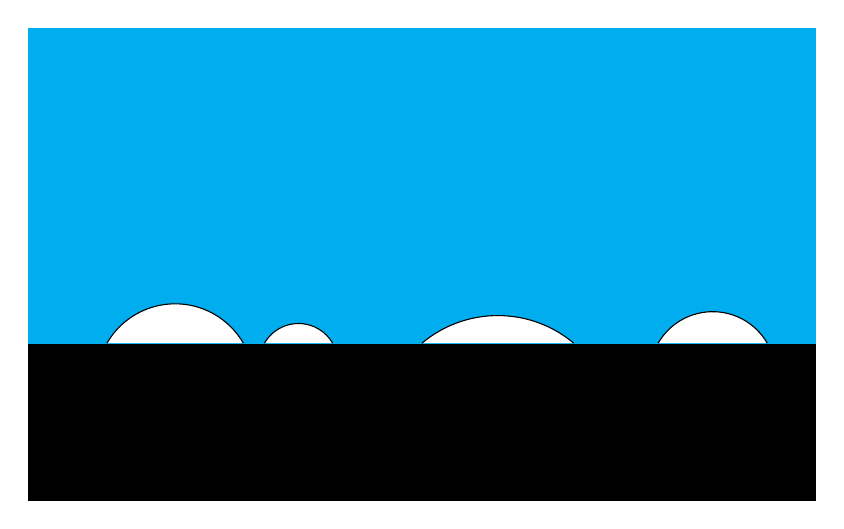
\begin{tikzpicture}
\filldraw (0,0) rectangle (10,-2);
\filldraw[color=cyan] (0,0) rectangle (10,4);

\draw[fill=white] (1,0) arc (150:30:1);
\draw[fill=white] (3,0) arc (150:30:0.5);
\draw[fill=white] (5,0) arc (130:50:1.5);
\draw[fill=white] (8,0) arc (150:30:0.8);

\end{tikzpicture}
\end{center}

The question naturally arises: when are nanobubbles present?  Yang and coworkers published in 2007 \cite{Yang2007} an exhaustive experimental study on the factors influencing the formation of nanobubbles, such as temperature, dissolved gases etc.  It turns out that if a surface had been immersed in ethanol before being immersed in water, then nanobubbles are reliably formed.  Using this `solvent exchange' technique, Yang and coworkers were able to do repeatable studies of nanobubbles.  Using infrared spectroscopy, they confirmed the presence of a gas phase 5 -- 80 nm thick at the surface --- i.e. good evidence that the `soft domains' really are nanobubbles.  The pressure in the bubbles was found to be 1.0 -- 1.7 atmospheres, consistent with the Laplace pressure calculated from their radii of curvature.  This low pressure allows nanobubbles of air to remain stable for days.  They find that nanobubbles form much more easily on rough surfaces, sometimes even without the solvent exchange technique.

Crucially, the solvent exchange technique is also a common cleaning technique.  Therefore, nanobubbles may be formed inadvertently in the process of a slip experiment.  Given the further fact that rough surfaces may spontaneously form nanobubbles, the question arises:  How many ostensibly `pure' slip experiments are actually experiments on \emph{mixed-slip} surfaces?

A purpose of the research in this thesis is to give some indication of the effect of such nanobubble contamination on a slip experiment.

\vspace*{1em}
In summary, mixed-slip surfaces tend to fall into the two types described above: either a solid surface interspersed with pockets of air (nanobubble type), or a gas-liquid interface interspersed with islands of solid material (superhydrophobic type).  Thus, a superhydrophobic type surface has a contiguous \emph{air-liquid} interface, while a nanobubble type surface has a contiguous \emph{solid} phase.

In the two-dimensional case, the difference disappears.  \emph{Neither} the solid-liquid nor air-liquid interfaces are contiguous.  Physically, this surface consists of a grating of parallel ridges, with an air gap between the ridges.  The liquid sits on the top of the ridges, and the air-liquid interface forms a meniscus between the ridges.


\section{Rough Surfaces}

In the previous section on mixed-slip surfaces, we focused on two archetypes drawn from the real world.  In keeping with their real-world nature, they have a hugely important feature: \emph{they are not flat.}  In a previous section, the slip length of a mixed-slip surface was defined with respect to a mathematically perfect \emph{flat plane.}  The definition of the slip length of a \emph{rough} surface is ambiguous.  The question ``What is the slip length of this surface?" suddenly acquires a resonance with the old Vaudeville joke ``How's your wife?";  the answer: ``Compared to what?".

To clarify, a surface with slip behaves as if the no-slip boundary was located some distance --- the slip length --- below the true surface.  For convenience, the plane $z=0$ in the mathematical model maps to the true surface. But for a rough surface, the physical position of $z=0$ is a matter of choice.  It could be reasonably defined to be at the highest point of the roughness, or the lowest point of the roughness, or at any point in between.  Put another way, a rough material has a  `nominal surface', which has some non-zero width --- essentially the distance between its lowest and highest points.  If a rough surface has a slip length that is  large compared to this surface width, then all is well, the slip length will be quoted with a small uncertainty equal to this ambiguity.  But slip lengths may be of the order of the width of the nominal surface.  In this case, the very existence of slip has disappeared into uncertainty about the surface location.


\begin{center}
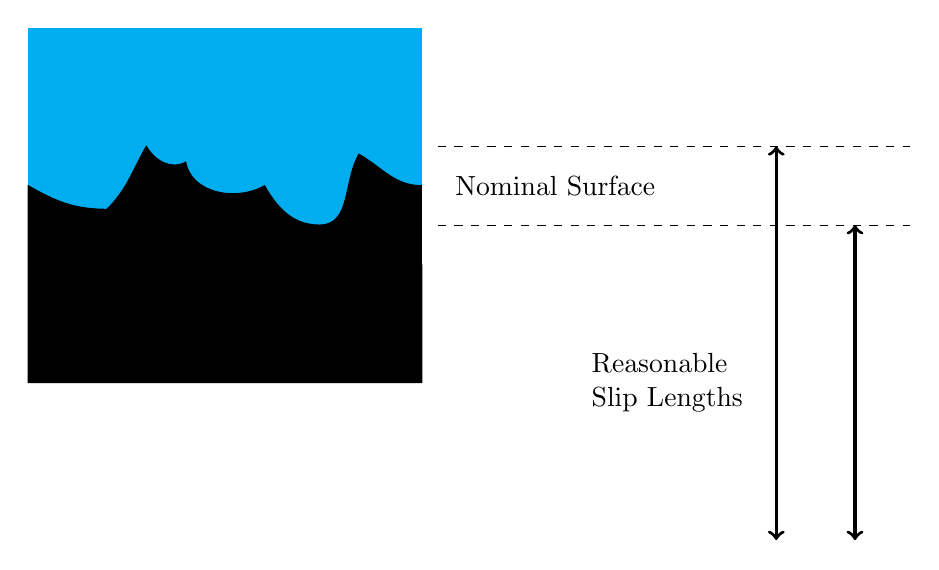
\begin{tikzpicture}
\draw[cyan, fill=cyan] (0,0) rectangle (5,3);

\filldraw (5,0) -- (5,-1.5) -- (0,-1.5) -- (0,1)  to [out=-30,in=180] 
          (1,0.7) to [out=45,in=240] (1.5,1.5)  to [out=-60,in=210] (2,1.3)
           to [out=-80,in=210] (3, 1)  to [out=-60,in=180] (3.7,0.5)
            to [out=0,in=240] (4.2,1.4)  to [out=-30,in=180] (5,1);
            
\draw[dashed] (5.2,0.5) -- +(6,0);
\draw[dashed] (5.2,1.5) -- +(6,0);

\node at (5.3,1)[right]{Nominal Surface};

\draw [<->,very thick] (9.5,1.5) -- +(0,-5);
\draw [<->,very thick] (10.5,0.5) -- +(0,-4);

\node at (9.2,-1.5) [left, align=left] {Reasonable\\ Slip Lengths};

\end{tikzpicture}
\end{center}

Surprisingly, a failure to consider the precise location of the $z=0$ point led to considerable confusion and contradiction in the early experimental literature on slip.

\vspace*{1em}

Studies were made on the effects of roughness on slip.  These involve a surface that is non-flat, but otherwise homogeneous; the material is the same everywhere, so is assumed to have the same intrinsic slip length everywhere.

\vspace*{1em}

In 2002, Zhu and Granick published results of drainage force experiments on hydrophobic surfaces of varying roughness \cite{ZhuGranick2002}.  The molecularly smooth surface showed a flow dependent slip length of up to 35 nm, while rougness \emph{suppressed} slip, with a roughness of 6 nm giving no slip at all.

They defined the $z=0$ level in the surface force appartatus by `adhesive contact in air'.  Therefore, the $z=0$ level could well be below the tops of the roughness peaks.  No effort was made to account for this.


A paper from 2003 by Bonaccurso, Butt and Craig \cite{BonaccursoButtCraig2003} claimed that roughness could \emph{increase} slip, even on a \emph{hydrophilic} (contact angle zero!) surface.
They measure drainage forces of a glass sphere approaching a silicon surface roughened up to 12.2 nm rms.

They discuss the importance of defining the zero distance.  They end up defining it at the tops of the peaks, as this is the first point of contact.  They calculate slip lengths by fitting the data to Vinogradova's model.  The best fit is when they fix the slip length on the glass sphere at about 43 nm, and increase the slip length of the substrate as roughness increases.  Under `normal' conditions, they find a slip length of 3.5 nm for maximum roughness of 12.2 nm.  But for extremely high approach velocities, for the same roughness they find a slip length of 900 nm!

Vinogradova herself waded into the issue in 2006, with a paper with Yakubov \cite{VinogradovaYakubov2006}.  They used a purpose-built AFM device that tapped a roughened sphere onto a smooth plane.  The sphere had an rms roughness of 10 -11 nm, and a maximum peak-to-valley distance of 45 nm.  With the surface taken to be at the tops of the peaks, a reduction in drainage force was observed, compared to a smooth sphere of equal diameter.  But the reduction was not due to slip:  The force was equivalent to that of a smooth sphere whose surface was located at an intermediate position between the peaks and valleys of the roughness.

Thus the issue is resolved: if the boundary is taken to be at the valleys of the roughness, then roughness reduces slip.  Conversely, if the boundary is taken to be at the tops of the peaks, then roughness \emph{increases} slip.
They note ``We believe our paper entirely clarifies the situation with flow past rough surfaces, highlights reasons for existing controversies, and resolves apparent paradoxes." 

A couple of numerical studies expand on Vinogradova's clarification.

Kunert and Harting in 2007 \cite{KunertHarting2007} formalized the concept with the introduction of an `effective no slip plane', typically located between the peaks and valleys of the surface roughness.  They carried out numerical simulations using lattice Boltzmann methods on different surfaces.  Each surface has minimum and maximum heights, $h_{\mathrm{min}}$ and $h_{\mathrm{max}}$, and an average height $h_{\mathrm{average}}$.  They calculate the position of the effective no-slip plane, $h_{\mathrm{eff}}$.  In all cases, $h_{\mathrm{eff}}$ was always considerably higher than $h_{\mathrm{average}}$.  If the surface has a few very tall but sparsely distributed spikes, then $h_{\mathrm{average}}$ can be much smaller than $h_{\mathrm{max}}$, and $h_{\mathrm{eff}}$ lies somewhere between them and cannot be well approximated by either.

In 2010 the same authors teamed up with Vinogradova \cite{KunertHartingVinogradova2010} to carry out lattice Boltzmann simulations of high-speed drainage between a smooth sphere and a randomly rough plane.  A sphere of radius $R$ approaches the plane $z=0$ located at the tops of the roughness.  Assuming that the plane $z=0$ has a single constant slip length, then asymptotically, the drainage force
\[ F \rightarrow \frac{9R}{32z} \quad \text{as} \;\;\; z \rightarrow 0 \]

Alternatively, assuming there is a no-slip plane located a distance $s$ below the top of the roughness,
\[ F \rightarrow \frac{9R}{8s} \quad \text{as} \;\;\; z \rightarrow 0 \]

At distant separations, the two models agree with each other, but at close separations, the forces predicted by the slip model are higher than observed, while the effective no-slip plane model fits the data very well.  

\vspace*{1em}

Hence, an effective no-slip plane located between the peaks and valleys of the roughness does a better job at explaining drainage forces than a slip boundary located on top of the roughness.  This is not surprising, since the drainage force of a sphere touching a surface (even with slip) will diverge, while the effective no-slip plane model always allows a finite space for fluid to escape.

However, for Couette or Poiseuille type flow, the two models should be equivalent; that is after all, one way of defining the slip length.  The important thing is to locate the effective no-slip plane.  The distance from there to the surface defined as $z=0$ determines the slip length.  These considerations are obviously still  important for any rough surface that also happens to be mixed-slip.

\begin{center}
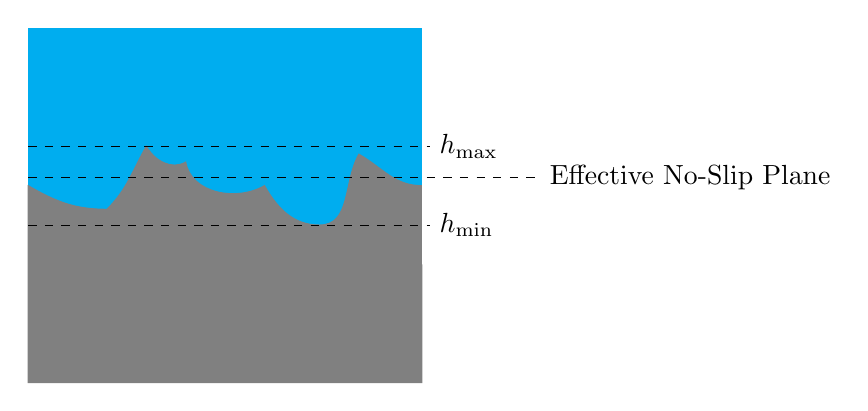
\begin{tikzpicture}

\draw[cyan, fill=cyan] (0,0) rectangle (5,3);

\filldraw [color=gray] (5,0) -- (5,-1.5) -- (0,-1.5) -- (0,1)  to [out=-30,in=180] 
          (1,0.7) to [out=45,in=240] (1.5,1.5)  to [out=-60,in=210] (2,1.3)
           to [out=-80,in=210] (3, 1)  to [out=-60,in=180] (3.7,0.5)
            to [out=0,in=240] (4.2,1.4)  to [out=-30,in=180] (5,1);
            
\draw[dashed] (0,0.5) -- +(5.1,0);
\draw[dashed] (0,1.5) -- +(5.1,0);
\node at (5.1,0.5)[right]{$h_{\mathrm{min}}$};
\node at (5.1,1.5)[right]{$h_{\mathrm{max}}$};

\draw[dashed] (0, 1.1) -- +(6.5,0);

\node at (6.5,1.1)[right]{Effective No-Slip Plane};

\end{tikzpicture}
\end{center}



\section{Mixed Slip Flow}

In 2003, Cottin-Bizonne \emph{et al} published a paper \cite{Cottin-Bizonne2003} in which they stated ``Our results show for the first time that, in contrast to common belief, surface friction may be reduced by surface roughness."  In fact, what they discovered is that flow over a rough surface may transition into the superhydrophobic state, with the fluid now flowing over vapour pockets.  (As previously stated, later that same year, Bonaccurso, Butt and Craig \cite{BonaccursoButtCraig2003} experimentally demonstrated that roughness increases slip. But they did not explicitly consider that their system may have entered the superhydrophobic regime.  Had it?)

Cottin-Bizonne and coworkers looked at molecular dynamics simulations of a Lennard-Jones fluid flowing over a flat surface decorated with narrow square posts.  At sufficiently low pressures, the fluid entered the Cassie state, as a vapour phase spontaneously formed at the surface, leaving the fluid supported on top of the posts.  The surface had an intrinsic slip length of 20 - 25 $\sigma$ (atom diameters).  In the Cassie state, slip lengths up to 57 $\sigma$ appeared.  For very narrow posts -- 4.9 $\sigma$, slip lengths could reach 130 $\sigma$.  Note that slip lengths were measured from the bottom of the cavity, so the post height --- 6 $\sigma$ --- could be added to the slip lengths.


A physical experiment of this superhydrophobic Cassie state flow was presented by Choi and Kim in 2006 \cite{ChoiKim2006}.  They were probably the first to deliberately engineer a surface for maximum slip: `nanoturf', silicon nanoposts about 1 - 2 $\mu$m high, spaced about 0.5 - 1.0 $\mu$m apart, rendered hydrophobic by a 10 - 20 nm thick layer of Teflon.  They estimated the air fraction of the surface to be 60 \%.

A commercial cone-and-plate rheometer was used to measure slip lengths: a collosal 20 $\mu$m for water and 50 $\mu$ for 30 \% glycerine solution.  (They expect this, since the viscosity of the glycerine solution is 2.5 times greater than that of water.)

Such suspiciously high slip lengths were not replicated in a more careful study by Joseph \emph{et al} also in 2006 \cite{Joseph2006}.  They did particle image velocimetry on channels coated with carbon nanotubes of diameter 50 - 100 nm, spaced 100 - 250 nm apart.  The tops of the nanotubes could be evenly spaced, or clumped together like wet hair, giving inter-clump length scales of 1.7, 3.5 or 6 $\mu$m.  The derived slip lengths for the three surface morphologies were roughly 0.4, 1.0 and 1.4 $\mu$m, respectively.

They note that their results are an order of magnitude smaller than the 20 $\mu$m slip lengths of Choi and Kim, and point out that rheological methods lack the sensitivity to measure surface effects.

An amusing effort was made by Lee and Kim in 2011 \cite{LeeKim2011} to maximize slip by making a heirarchical structured surface --- nanoposts on top of microposts.  It worked if area fraction taken up by the microposts was large enough.  Below about 10\% area fraction --- a realistic figure --- the advantage began to disappear, and at 4\% area fraction, the heirarchical surface gave \emph{lower} slip than conventional unadorned microposts.

\vspace*{1em}

A one-dimensional version of the superhydrophobic surface is a nanograting --- a surface covered with ridges, with the water supported by surface tension on top of the ridges.  In 2006, Choi \emph{et al} \cite{Choi2006} presented slip experiments on a ``well-defined nanograte": ridges 500 nm high and 50 nm wide, separated by a gap of 180 nm.  Thus the pitch (period) was 230 nm.
If the grating was left hydrophilic, they believe that water fully wets the surface, penetrating down into the troughs.  After rendering the surface hydrophobic with Teflon, they believe that there is air in the troughs.  Experiments were carried out with both states, with fluid flow both parallel to, and transverse to the ridges.

They could measure slip lengths to a resolution of only 30 nm, thus they were unsure if the hydrophobic surface had any intrinsic slip.  For flow parallel to the ridges, there was a clear distinction between the slip lengths of hydrophilic and hydrophobic surfaces.  $30 \pm 15$ nm for hydrophilic, and $143 \pm 35$ nm for hydrophobic.  For transverse flow, they found insignificant slip, $0 \pm 17$ for hydrophilic, and $61 \pm 44$ for hydrophobic.

\vspace*{1em}

One can imagine the difficulties in studying a surface of nanobubbles, given their random, uncontrolled nature.  Steinberger \emph{et al} in 2007 \cite{Steinberger2007} addressed the issue by studying flow over a flat surface covered with holes 1.3 $\mu$m wide and 3.5 $\mu$m deep.  Air can be trapped in the holes; they derive slip lengths via drainage force measurements on the resulting microbubble surface.

The plane $z=0$ is located on the flat surface, at the tops of the holes.  In the Wenzel state, with water filling the holes, they measure a slip length of $105 \pm 10$ nm.  With air trapped in the holes, bizarrely, they find a \emph{lower} slip length: a mere $20 \pm 10$ nm.  Understandably, they are puzzled by this, so they invsetigate.  They discover that the microbubbles protrude an estimated 200 - 400 nm above the flat surface, with the meniscus subtending an angle between $30^{\circ}$ and $60^{\circ}$ to the flat surface.  Is this protrusion into the bulk the cause of low slip lengths?

They test this hypothesis numerically, with a finite element package (Comsol).  They find a flat bubble ($\theta = 0^{\circ}$) gives maximum slip length --- about 160 nm.  Any increase in $\theta$ decreased slip, with $\theta > 45^{\circ}$ giving a lower slip length than the Wenzel state.

The following year (2008) Hyv\"{a}luoma and Harting replicate and extend Steinberger's numerics \cite{HyvaluomaHarting2008}.  By using lattice Boltzmann methods, they can model the bubble deforming under stress.  They essentially replicate Steinberger: a maximum slip of about 150 nm at zero protrusion angle, plummeting down past zero slip length for a protrusion angle greater than about $70^{\circ}$

They simulate Couette flow, so are able to investigate shear dependence.  In steady state shear-driven flow, they see a \emph{decrease} in slip length with increasing shear.  This contradicts some earlier claims.  However, higher shear rates deform the microbubbles, reducing the average height of the microbubbles.

They claim that this is consistent with Kunert and Harting 2007 \cite{KunertHarting2007}, which showed reduced slip from reduced roughness.
However a careful reading sheds doubt on this. The upshot of Kunert and Harting 2007 \cite{KunertHarting2007} is that if the peaks are lowered, then the position of the effective no-slip plane will be lowered too, but \emph{not as much.}  Thus, there is a reduced distance from the effective no-slip plane to the $z=0$ plane \emph{on the tops of the roughness peaks.} Put another way, the effective no-slip plane has actually \emph{risen} with respect to the $z=0$ plane. That is to say, the slip length has reduced (caused by reduced roughness).  


\begin{center}
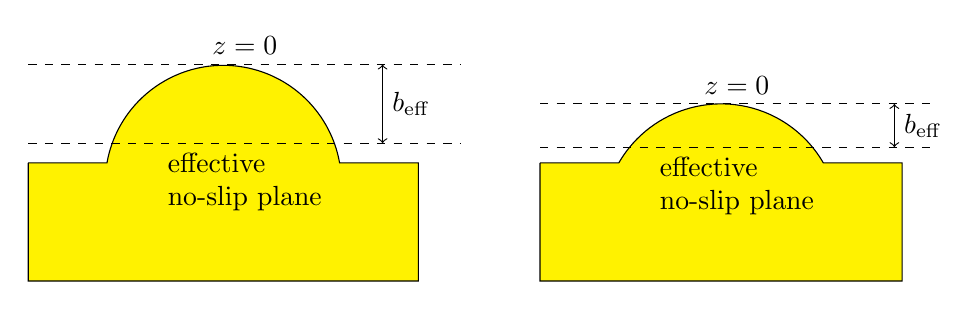
\begin{tikzpicture}

\path (0,0) coordinate (orig1);
\path (6.5,0) coordinate (orig2);

\draw[fill=yellow] (orig1) -- ++(1,0) arc(170:10:1.5) -- ++(1,0) --++(0,-1.5) -| (orig1);
\draw[dashed] (orig1) ++(0,1.25) -- node [above] {$z=0$} ++(5.5,0) ;
\draw[dashed] (orig1) ++(0,0.25) -- node [below,align=left]
{effective\\no-slip plane} ++(5.5,0);
\draw[<->] (orig1) ++(4.5,0.25) -- node[right]{\beff} ++(0,1);

\draw[fill=yellow] (orig2) -- ++(1,0) arc(150:30:1.5) -- ++(1,0) --++(0,-1.5) -| (orig2);
\draw[dashed] (orig2) ++(0,0.75) -- node [above] {$z=0$} ++(5,0) ;
\draw[dashed] (orig2) ++(0,0.2) -- node [below,align=left]
{effective\\no-slip plane} ++(5,0);
\draw[<->] (orig2) ++(4.5,0.2) -- node[right]{\beff} ++(0,0.55);

\end{tikzpicture}
\end{center}

However, in Hyv\"{a}luoma and Harting 2008 \cite{HyvaluomaHarting2008}, the $z=0$ plane is at the `top of the structured surface' which seems to mean the \emph{bottom} of the roughness.  In that case, a lowered effective no-slip plane (for any reason), is always lower with respect to the $z=0$ plane, which is equivalent to \emph{increased} slip length.  (If the effective no-slip plane was above the $z=0$ plane to start with, then the slip length becomes \emph{less negative.})

\begin{center}
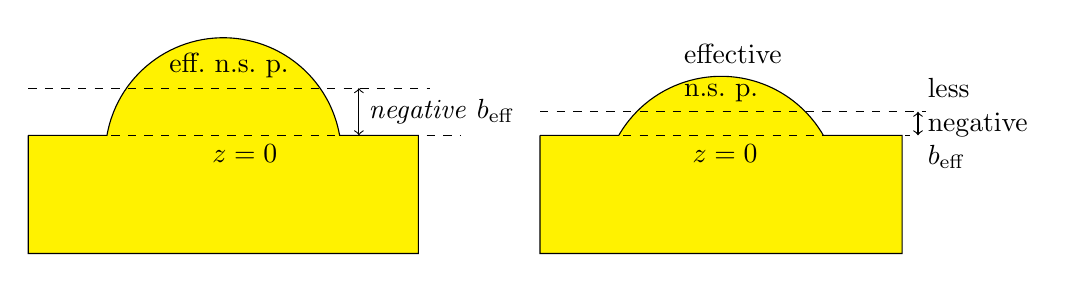
\begin{tikzpicture}

\path (0,0) coordinate (orig1);
\path (6.5,0) coordinate (orig2);

\draw[fill=yellow] (orig1) -- ++(1,0) arc(170:10:1.5) -- ++(1,0) --++(0,-1.5) -| (orig1);
\draw[dashed] (orig1) -- node [below] {$z=0$} ++(5.5,0) ;
\draw[dashed] (orig1) ++(0,0.6) -- node [above] {eff.\ n.s.\ p.} ++(5.1,0);
\draw[<->] (orig1) ++(4.2,0) -- node[right]{\emph{negative} \beff} ++(0,0.6);

\draw[fill=yellow] (orig2) -- ++(1,0) arc(150:30:1.5) -- ++(1,0) --++(0,-1.5) -| (orig2);
\draw[dashed] (orig2) -- node [below] {$z=0$} ++(4.7,0) ;
\draw[dashed] (orig2) ++(0,0.3) -- node [above,align=left]
{effective\\n.s.\ p.} ++(4.9,0);
\draw[<->] (orig2) ++(4.8,0) -- node[right,align=left]{less\\negative\\ \beff} ++(0,0.3);

\end{tikzpicture}
\end{center}

So, the increase in slip from reduced bubble height seems not to be consistent with Harting's earlier work with Kunert.  Instead, I hypothesize that a deformed bubble has a steeper wall on the downstream side, causing more stagnancy and turbulence in the lee of the bubble, thus a lower average surface velocity, hence a lower slip length.

\begin{center}
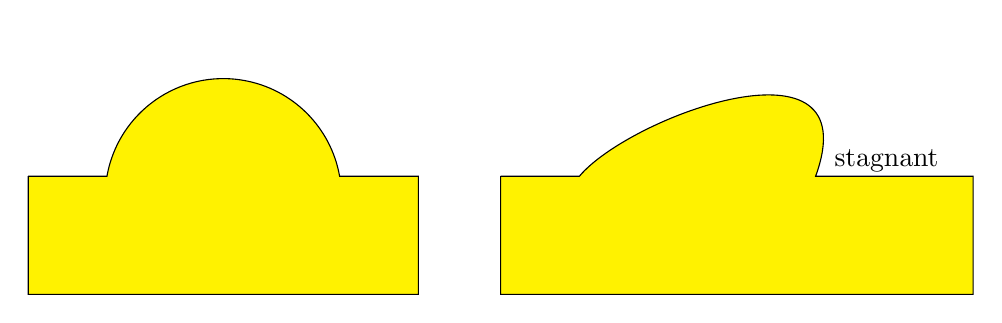
\begin{tikzpicture}

\path (0,0) coordinate (orig1);
\path (6,0) coordinate (orig2);

\draw[fill=yellow] (orig1) -- ++(1,0) arc(170:10:1.5) -- ++(1,0) --++(0,-1.5) -| (orig1);

%\draw[fill=yellow] (orig2) -- ++(1,0) to [out=60,in=180]  ++(2,1) to [out=0,in=60]
% ++(1,-1) -- ++(2,0) -- ++(0,-1.5) -| (orig2);

\draw[fill=yellow] (orig2) -- ++(1,0) .. controls +(50:1) and +(70:2) .. ++(3,0)
 -- ++(2,0) -- ++(0,-1.5) -| (orig2);

\path (orig2) ++(4.9,0.2) node {stagnant};

\end{tikzpicture}
\end{center}


Incidentally, the idea that slip is reduced by protruding bubbles had been proposed by Lauga and Brenner in 2004 \cite{LaugaBrenner2004}.  In a theoretical paper, they present a model to explain the shear-dependent slip found by Zhu and Granick in 2001 \cite{ZhuGranick2001}.  They assume that the surface was (unknown to the experimenters) covered in bubbles.  Slip lengths were inferred from the drainage force of a probe slamming into the surface at various speeds. As the probe approach velocity increases, so too does the pressure in front of it.  This increased pressure causes the bubbles to shrink, both from compression of the gas and increased diffusion into the liquid.  The reduced bubble height widens the channel, making drainage easier, for a given probe-surface distance.  Thus, this `leaking mattress effect' causes a
\nopagebreak[0] shear-dependent slip effect to appear.

\vspace{3em}

In summary, high slip lengths are possible over mixed-slip surfaces: more than 100 nanometers for nanogratings, and more than 1 micron for nanoforests.  However, the effective slip length has a slightly ambiguous definition; the quoted slip length depends on the nominal position of the $z=0$ plane.  Things are clarified by introducing the concept of an effective no-slip plane.  This is an objective concept: the surface behaves as if the no-slip plane was located at a given position.  Then, the slip length is the distance between $z=0$ and the effective no-slip plane.  Thus, if the no-slip plane becomes lower, then the slip length is increased, and vice versa.  A sensible choice for the position of the nominal $z=0$ plane is the \emph{top of the roughness.}  That way, quoted slip lengths will often be positive.  Note that if the $z=0$ plane was chosen to be \emph{below} the no-slip plane to start with, lowering the no-slip plane still \emph{increases} the slip length by making it \emph{less negative.}


\clearpage

\section{Effective Slip Lengths}


There are a small number of results for effective slip lengths in the literature.  In this section, we survey a dozen or so of them.  This cannot pretend to be comprehensive --- there may be results hidden in obscure journals, behind paywalls, or camouflaged by nonstandard terminology.  Further, mathematically equivalent results may exist in fields unrelated to fluid mechanics.  There is nothing we can do about this.  The best we can claim to do is present some `high profile' results in the field of fluid slip.

\subsection*{Categorizing Results by Regime of Applicability}

The published results for an effective slip length are applicable in different physical situations.  It is useful to sort these different regimes by the following criteria:

\begin{itemize}

\item \textbf{Navier Stokes} versus \textbf{Stokes}.  A few results use the full Navier Stokes description of fluid flow.  However, slip is very small scale phenomenon, so the characteristic length scale of the flow is also very small.  Thus, the Reynolds number is very small, and the Navier Stokes equation is very well approximated by the simpler Stokes flow equation.  (This is covered fully in the next chapter.)  Accordingly, most results have been derived assuming only Stokes `creeping' flow.

\item \textbf{Flat} versus \textbf{Rough}. Assuming the boundary to be the flat plane $z=0$ is a major simplification, warranted on grounds of mathematical tractability.  Two thirds of effective slip results make this assumption.

\item \textbf{2-D Flow} (1-D Surface) versus \textbf{3-D Flow} (2-D Surface).
If the surface is symmetric in one dimension, then the flow above it will have the same symmetry.  Thus, full three-dimensional flow reduces to two-dimensional flow over a one-dimensional surface pattern.  About half of effective slip results tackle this simpler case.

\item \textbf{Perfect-slip/Zero-slip Binary Surface} or \textbf{Not.}  Assuming a binary surface, comprising regions of either vanishing slip ($b=0$), or perfect slip ($b \rightarrow \infty$) only, can enable considerable simplification of the mathematics.  Half of all effective slip results tackle this limiting case.

\end{itemize}

These categories are used to construct Table \ref{table:slipresults}.  All the papers that we shall survey in this section appear in the table, in their appropriate categories.  Some papers appear in more than one cell; in that case, the paper presents more than one result.  Note that if a paper gives a \emph{single} result for a case that \emph{subsumes} another case (eg. a 3-D result that is automatically valid for the 2-D case), then the paper appears in only \emph{one} cell.


\begin{table}
\caption{The papers (presenting effective slip lengths) surveyed in this section, 
categorized into their applicable regimes.}
\label{table:slipresults}

\begin{center}
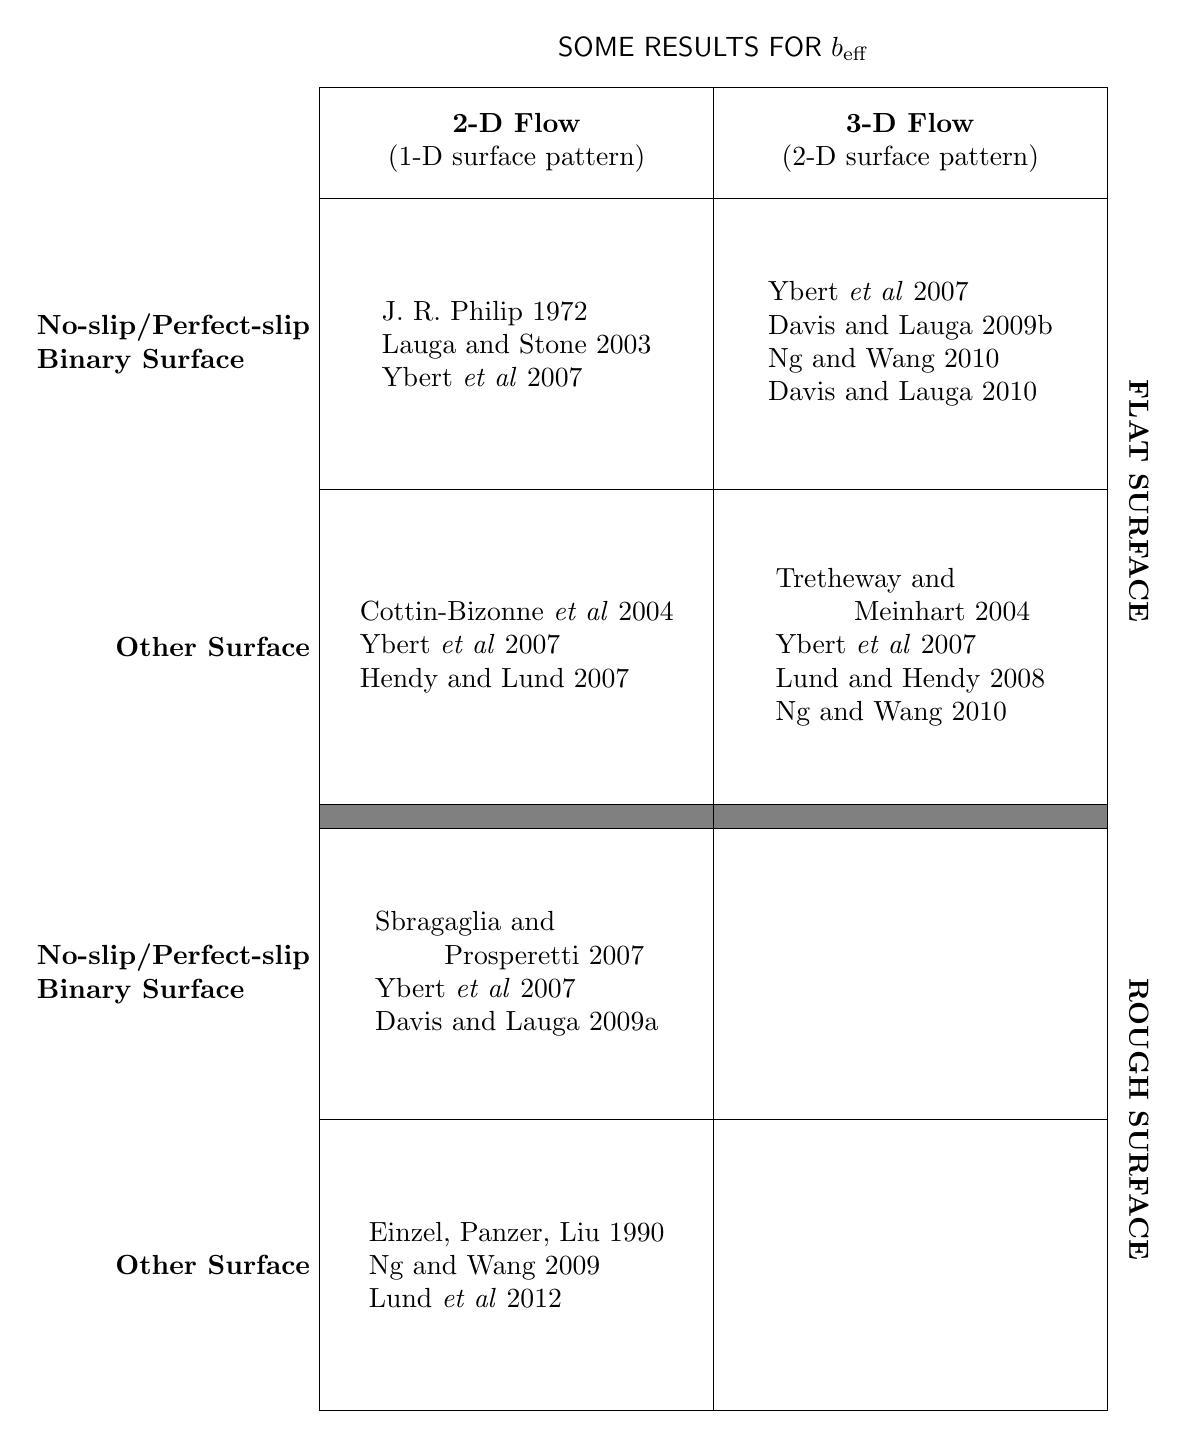
\begin{tikzpicture}

% Manually define half width of table.
\path (5,0) coordinate (midway);

% Manually define row heights.
\path (0,3.7) coordinate (flatbinary);
\path (0,4) coordinate (flatother);
\path (0,3.7) coordinate (roughbinary);
\path (0,3.7) coordinate (roughother);

\path (0,0.3) coordinate (sepwidth);

\path (0,1.4) coordinate (labelbox);

%%%%%%%%%%%%%%%%%%%%%%%%%%%%%%%%%%%%%%%%% Tikz calculates all other points...
% Bottom left corner is origin (0,0)
\path (0,0) ++(midway) coordinate (midbottom);

\path (0,0) ++(roughother) coordinate (lowdiv);
\path (lowdiv) ++(roughbinary) coordinate (belowsep);
\path (belowsep) ++(sepwidth) coordinate (abovesep);
\path (abovesep) ++(flatother) coordinate (highdiv);
\path (highdiv) ++(flatbinary) coordinate (celltop);
\path (celltop) ++ (labelbox) ++(midway) coordinate (topmid);
\path (topmid) ++(midway) coordinate (topright);


%%%%%%%%%%%%%%%%%%%%%%%%%%%%%%%%%%%%%%% Draw all boxes and lines...
\draw (0,0) rectangle (topright);
\draw (celltop) -- ++(midway) -- ++(midway);
\draw (highdiv) -- ++(midway) -- ++(midway);
\draw [fill=gray] (abovesep) ++(midway) ++(midway) rectangle (belowsep);
\draw (lowdiv) -- ++(midway) -- ++(midway);
\draw (topmid) -- (midbottom);

%%%%%%%%%%%%%%%%%%%%%%%%%%%%%%%%%%%%%%% Add flow type labels.
\path (celltop) --         coordinate[midway] (2Dlabel) (topmid);
\path (2Dlabel) ++(midway) coordinate (3Dlabel);
\node at (2Dlabel)[align=center] {\textbf{2-D Flow}\\(1-D surface pattern)};
\node at (3Dlabel)[align=center] {\textbf{3-D Flow}\\(2-D surface pattern)};

%%%%%%%%%%%%%%%%%%%%%%%%%%%%%%%%%%%%%%   Labels for surface types
\path (abovesep) -- coordinate[midway] (midflat) (celltop);
\path (0,0) --      coordinate[midway] (midrough) (belowsep);
\path (midflat) ++(midway) ++(midway) ++(0.4,0) coordinate (flatlabel);
\path (midrough) ++(midway) ++(midway) ++(0.4,0) coordinate (roughlabel);
\node at (flatlabel)  [rotate=270] {\textbf{FLAT SURFACE}};
\node at (roughlabel) [rotate=270] {\textbf{ROUGH SURFACE}};

%%%%%%%%%%%%%%%%%%%%%%%%%%%%%%%%%%%%%%%%%%%%%%%%%%%  Points in middle of rows...
\path (celltop)  -- coordinate[midway] (row1) (highdiv);
\path (highdiv)  -- coordinate[midway] (row2) (abovesep);
\path (belowsep) -- coordinate[midway] (row3) (lowdiv);
\path (lowdiv)   -- coordinate[midway] (row4) (0,0);

%%%%%%%%%%%%%%%%%%%%%%%%%%%%%%%%%%%%%%%%%%%%%%  Labels for Binary or Other surface types.
\node at (row1) [left, align=left] {\textbf{No-slip/Perfect-slip}\\
										\textbf{Binary Surface}};
\node at (row2) [left, align=left] {\textbf{Other Surface}};
\node at (row3) [left, align=left] {\textbf{No-slip/Perfect-slip}\\
										\textbf{Binary Surface}};
\node at (row4) [left, align=left] {\textbf{Other Surface}};

%%%%%%%%%%%%%%%%%%%%%%%%%%%%%%%%%%%%%%%%%%%%%%%%%  Locations of Text nodes...
%%%%%%%%%%%%  2-D Flow
\path (row1) -- coordinate[midway] (flatbin2D) +(midway);
\path (row2) -- coordinate[midway] (flatother2D) +(midway);
\path (row3) -- coordinate[midway] (roughbin2D) +(midway);
\path (row4) -- coordinate[midway] (roughother2D) +(midway);
%%%%%%%%%%%%%%  3-D Flow
\path (flatbin2D) ++(midway) coordinate (flatbin3D);
\path (flatother2D) ++(midway) coordinate (flatother3D);
\path (roughbin2D) ++(midway) coordinate (roughbin3D);
\path (roughother2D) ++(midway) coordinate (roughother3D);

%%%%%%%%%%%%%%%%%%%%%%%%%%%%%%%%%%%%%%%%%%%%%   LABEL FOR WHOLE TABLE
\path (topmid) ++(0,0.5) coordinate (heading);
\node at (heading) {\textsf{SOME RESULTS FOR \beff} };


%%%%%%%%%%%%%%%%%%%%%%%%%%%%%%%%%%%%%%%%%%%%%%%  Contents of Cells.....

\node at (flatbin2D) [align=left]
							{
							J. R. Philip 1972 \\
							Lauga and Stone 2003 \\
							Ybert \emph{et al} 2007
							};
							
\node at (flatbin3D) [align=left]
							{
							Ybert \emph{et al} 2007 \\
							Davis and Lauga 2009b \\
							Ng and Wang 2010 \\
							Davis and Lauga 2010
							};
							
\node at (flatother2D) [align=left]
							{
							Cottin-Bizonne \emph{et al} 2004 \\
							Ybert \emph{et al} 2007 \\
							Hendy and Lund 2007
							};
							
\node at (flatother3D) [align=left]
							{
							Tretheway and \\
								\phantom{mmm} Meinhart 2004 \\
							Ybert \emph{et al} 2007 \\
							Lund and Hendy 2008 \\
							Ng and Wang 2010
							};
							
\node at (roughbin2D) [align=left]
							{
							Sbragaglia and \\
								\phantom{mmm}Prosperetti 2007 \\
							Ybert \emph{et al} 2007 \\
							Davis and Lauga 2009a
							};

\node at (roughbin3D) [align=left]
							{
							
							};
							
\node at (roughother2D) [align=left]
							{
							Einzel, Panzer, Liu 1990 \\
							Ng and Wang 2009 \\
							Lund \emph{et al} 2012
							};

\node at (roughother3D) [align=left]
							{
							
							};
							
\end{tikzpicture}
\end{center}

\end{table}

\newpage


\subsection*{Categorizing Results by Mathematical Strength}

As well as sorting the published $\beff$ results by the regime of applicability, we can sort them by the rigour of their derivation.

Mathematicians may describe a result as `exact'.  This usually means that it is in a form that can be written down as an explicit formula.  The benefit of an exact result is practical: it can be evaluated more easily.  Whether a result is exact or not is nothing to do with the rigour of its derivation; i.e. unrelated to the \emph{strength} of the result. 

In mathematics, a result is described as \emph{strong} if \emph{few assumptions} were made in its derivation.  The fewer the assumptions, the `stronger' the result.
There are two benefits of a strong result: First, because it relies on fewer assumptions, it is likely to be more widely applicable.  `Strong' simply means `more general'.  Secondly, the fewer assumptions, the fewer modes of failure.  Assumptions some times turn out to be false; this sad event may cause various results to be overturned.  A strong result is more robust.  It is less fragile to nasty surprises as the body of human knowledge grows.  (Note that a strong result may have a long complicated derivation, and thus be vulnerable to errors in the derivation.  The point is that a stronger result has a more \emph{self contained} derivation.)

Obviously, in theoretical physics we would like our results to be as useful and trustworthy as possible --- `exact' and `strong'.  For the purposes of this literature review, we shall rank the published results using the following (somewhat arbitrary) labels.

\begin{itemize}

\item \textbf{Derived} Results.  A relation for $\beff$ derived (mathematically) from the Stokes equation, an appropriate boundary condition, and perhaps an assumption of fluid incompressibility.

\end{itemize}

Other results:

\begin{itemize}

\item \textbf{Scaling Law} Results.  May or may not include more assumptions than a Derived Result, but the result is not exact, giving $\beff$ only as a multiple of some other length scale.

\item \textbf{Simplified} Results.  Further simplifying assumptions have been made, from reasonable phenomenological models to mere hand waving.

\item \textbf{Empirical} Results.  Exact results that express a curve fitted to either numerical or experimental data.  May be informed by stronger results.

\end{itemize}


There are comparatively fewer Derived Results.  They are listed in Table \ref{table:derivedslip}.  The other results are listed in Table \ref{table:otherslip}.

\begin{table}
\caption{The papers surveyed here in which $\beff$ is rigorously derived from only the Stokes equation, an appropriate boundary condition and perhaps the assumption of fluid incompressibility.}
\label{table:derivedslip}

\begin{center}
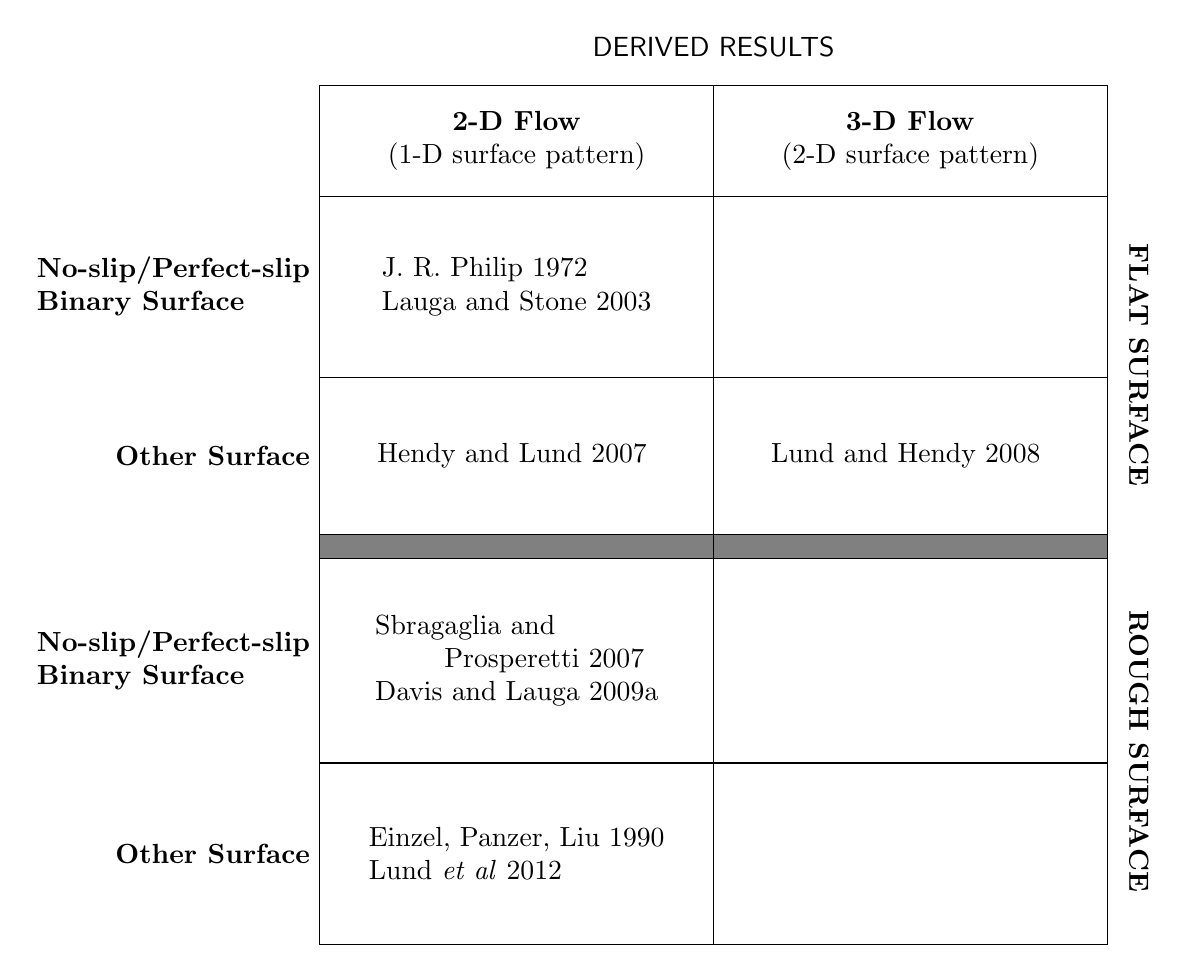
\begin{tikzpicture}

% Manually define half width of table.
\path (5,0) coordinate (midway);

% Manually define row heights.
\path (0,2.3) coordinate (flatbinary);
\path (0,2) coordinate (flatother);
\path (0,2.6) coordinate (roughbinary);
\path (0,2.3) coordinate (roughother);

\path (0,0.3) coordinate (sepwidth);

\path (0,1.4) coordinate (labelbox);

%%%%%%%%%%%%%%%%%%%%%%%%%%%%%%%%%%%%%%%%% Tikz calculates all other points...
% Bottom left corner is origin (0,0)
\path (0,0) ++(midway) coordinate (midbottom);

\path (0,0) ++(roughother) coordinate (lowdiv);
\path (lowdiv) ++(roughbinary) coordinate (belowsep);
\path (belowsep) ++(sepwidth) coordinate (abovesep);
\path (abovesep) ++(flatother) coordinate (highdiv);
\path (highdiv) ++(flatbinary) coordinate (celltop);
\path (celltop) ++ (labelbox) ++(midway) coordinate (topmid);
\path (topmid) ++(midway) coordinate (topright);


%%%%%%%%%%%%%%%%%%%%%%%%%%%%%%%%%%%%%%% Draw all boxes and lines...
\draw (0,0) rectangle (topright);
\draw (celltop) -- ++(midway) -- ++(midway);
\draw (highdiv) -- ++(midway) -- ++(midway);
\draw [fill=gray] (abovesep) ++(midway) ++(midway) rectangle (belowsep);
\draw (lowdiv) -- ++(midway) -- ++(midway);
\draw (topmid) -- (midbottom);

%%%%%%%%%%%%%%%%%%%%%%%%%%%%%%%%%%%%%%% Add flow type labels.
\path (celltop) --         coordinate[midway] (2Dlabel) (topmid);
\path (2Dlabel) ++(midway) coordinate (3Dlabel);
\node at (2Dlabel)[align=center] {\textbf{2-D Flow}\\(1-D surface pattern)};
\node at (3Dlabel)[align=center] {\textbf{3-D Flow}\\(2-D surface pattern)};

%%%%%%%%%%%%%%%%%%%%%%%%%%%%%%%%%%%%%%   Labels for surface types
\path (abovesep) -- coordinate[midway] (midflat) (celltop);
\path (0,0) --      coordinate[midway] (midrough) (belowsep);
\path (midflat) ++(midway) ++(midway) ++(0.4,0) coordinate (flatlabel);
\path (midrough) ++(midway) ++(midway) ++(0.4,0) coordinate (roughlabel);
\node at (flatlabel)  [rotate=270] {\textbf{FLAT SURFACE}};
\node at (roughlabel) [rotate=270] {\textbf{ROUGH SURFACE}};

%%%%%%%%%%%%%%%%%%%%%%%%%%%%%%%%%%%%%%%%%%%%%%%%%%%  Points in middle of rows...
\path (celltop)  -- coordinate[midway] (row1) (highdiv);
\path (highdiv)  -- coordinate[midway] (row2) (abovesep);
\path (belowsep) -- coordinate[midway] (row3) (lowdiv);
\path (lowdiv)   -- coordinate[midway] (row4) (0,0);

%%%%%%%%%%%%%%%%%%%%%%%%%%%%%%%%%%%%%%%%%%%%%%  Labels for Binary or Other surface types.
\node at (row1) [left, align=left] {\textbf{No-slip/Perfect-slip}\\
										\textbf{Binary Surface}};
\node at (row2) [left, align=left] {\textbf{Other Surface}};
\node at (row3) [left, align=left] {\textbf{No-slip/Perfect-slip}\\
										\textbf{Binary Surface}};
\node at (row4) [left, align=left] {\textbf{Other Surface}};

%%%%%%%%%%%%%%%%%%%%%%%%%%%%%%%%%%%%%%%%%%%%%%%%%  Locations of Text nodes...
%%%%%%%%%%%%  2-D Flow
\path (row1) -- coordinate[midway] (flatbin2D) +(midway);
\path (row2) -- coordinate[midway] (flatother2D) +(midway);
\path (row3) -- coordinate[midway] (roughbin2D) +(midway);
\path (row4) -- coordinate[midway] (roughother2D) +(midway);
%%%%%%%%%%%%%%  3-D Flow
\path (flatbin2D) ++(midway) coordinate (flatbin3D);
\path (flatother2D) ++(midway) coordinate (flatother3D);
\path (roughbin2D) ++(midway) coordinate (roughbin3D);
\path (roughother2D) ++(midway) coordinate (roughother3D);

%%%%%%%%%%%%%%%%%%%%%%%%%%%%%%%%%%%%%%%%%%%%%   LABEL FOR WHOLE TABLE
\path (topmid) ++(0,0.5) coordinate (heading);
\node at (heading) {\textsf{DERIVED RESULTS} };


%%%%%%%%%%%%%%%%%%%%%%%%%%%%%%%%%%%%%%%%%%%%%%%  Contents of Cells.....

\node at (flatbin2D) [align=left]
							{
							J. R. Philip 1972 \\
							Lauga and Stone 2003
							};
							
\node at (flatbin3D) [align=left]
							{
							};
							
\node at (flatother2D) [align=left]
							{
							Hendy and Lund 2007
							};
							
\node at (flatother3D) [align=left]
							{
							Lund and Hendy 2008
							};
							
\node at (roughbin2D) [align=left]
							{
							Sbragaglia and \\
								\phantom{mmm}Prosperetti 2007 \\
							Davis and Lauga 2009a
							};

\node at (roughbin3D) [align=left]
							{
							
							};
							
\node at (roughother2D) [align=left]
							{
							Einzel, Panzer, Liu 1990 \\
							Lund \emph{et al} 2012
							};

\node at (roughother3D) [align=left]
							{
							
							};
							
\end{tikzpicture}
\end{center}

\end{table}


%\vspace*{2em}

\begin{table}
\caption{The papers surveyed here in which $\beff$ is not exact, or does not have a rigorous derivation.}
\label{table:otherslip}

\begin{center}
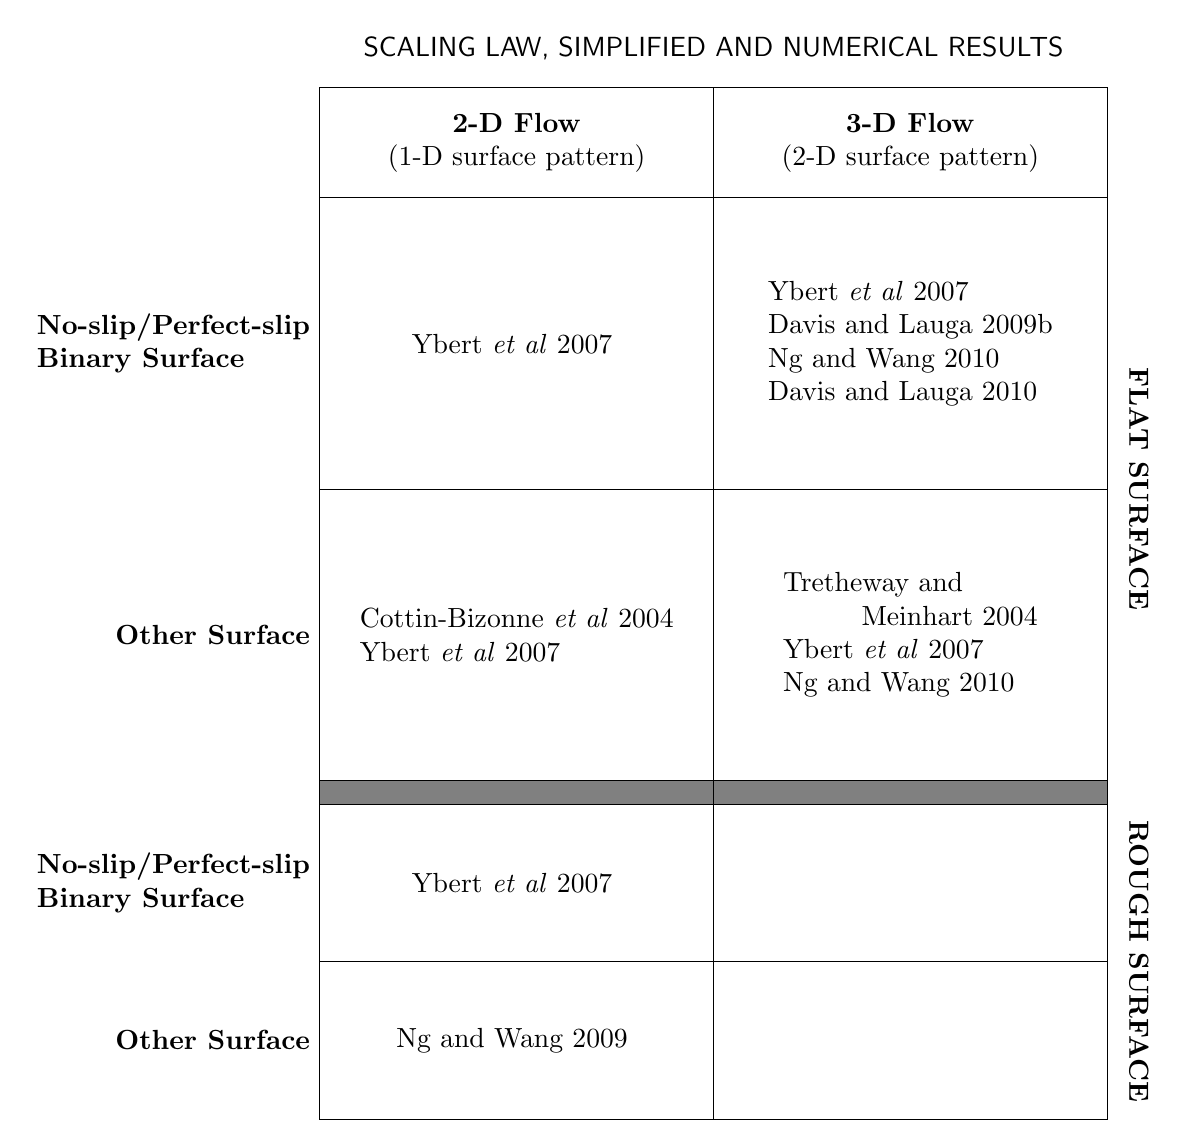
\begin{tikzpicture}

% Manually define half width of table.
\path (5,0) coordinate (midway);

% Manually define row heights.
\path (0,3.7) coordinate (flatbinary);
\path (0,3.7) coordinate (flatother);
\path (0,2) coordinate (roughbinary);
\path (0,2) coordinate (roughother);

\path (0,0.3) coordinate (sepwidth);

\path (0,1.4) coordinate (labelbox);

%%%%%%%%%%%%%%%%%%%%%%%%%%%%%%%%%%%%%%%%% Tikz calculates all other points...
% Bottom left corner is origin (0,0)
\path (0,0) ++(midway) coordinate (midbottom);

\path (0,0) ++(roughother) coordinate (lowdiv);
\path (lowdiv) ++(roughbinary) coordinate (belowsep);
\path (belowsep) ++(sepwidth) coordinate (abovesep);
\path (abovesep) ++(flatother) coordinate (highdiv);
\path (highdiv) ++(flatbinary) coordinate (celltop);
\path (celltop) ++ (labelbox) ++(midway) coordinate (topmid);
\path (topmid) ++(midway) coordinate (topright);


%%%%%%%%%%%%%%%%%%%%%%%%%%%%%%%%%%%%%%% Draw all boxes and lines...
\draw (0,0) rectangle (topright);
\draw (celltop) -- ++(midway) -- ++(midway);
\draw (highdiv) -- ++(midway) -- ++(midway);
\draw [fill=gray] (abovesep) ++(midway) ++(midway) rectangle (belowsep);
\draw (lowdiv) -- ++(midway) -- ++(midway);
\draw (topmid) -- (midbottom);

%%%%%%%%%%%%%%%%%%%%%%%%%%%%%%%%%%%%%%% Add flow type labels.
\path (celltop) --         coordinate[midway] (2Dlabel) (topmid);
\path (2Dlabel) ++(midway) coordinate (3Dlabel);
\node at (2Dlabel)[align=center] {\textbf{2-D Flow}\\(1-D surface pattern)};
\node at (3Dlabel)[align=center] {\textbf{3-D Flow}\\(2-D surface pattern)};

%%%%%%%%%%%%%%%%%%%%%%%%%%%%%%%%%%%%%%   Labels for surface types
\path (abovesep) -- coordinate[midway] (midflat) (celltop);
\path (0,0) --      coordinate[midway] (midrough) (belowsep);
\path (midflat) ++(midway) ++(midway) ++(0.4,0) coordinate (flatlabel);
\path (midrough) ++(midway) ++(midway) ++(0.4,0) coordinate (roughlabel);
\node at (flatlabel)  [rotate=270] {\textbf{FLAT SURFACE}};
\node at (roughlabel) [rotate=270] {\textbf{ROUGH SURFACE}};

%%%%%%%%%%%%%%%%%%%%%%%%%%%%%%%%%%%%%%%%%%%%%%%%%%%  Points in middle of rows...
\path (celltop)  -- coordinate[midway] (row1) (highdiv);
\path (highdiv)  -- coordinate[midway] (row2) (abovesep);
\path (belowsep) -- coordinate[midway] (row3) (lowdiv);
\path (lowdiv)   -- coordinate[midway] (row4) (0,0);

%%%%%%%%%%%%%%%%%%%%%%%%%%%%%%%%%%%%%%%%%%%%%%  Labels for Binary or Other surface types.
\node at (row1) [left, align=left] {\textbf{No-slip/Perfect-slip}\\
										\textbf{Binary Surface}};
\node at (row2) [left, align=left] {\textbf{Other Surface}};
\node at (row3) [left, align=left] {\textbf{No-slip/Perfect-slip}\\
										\textbf{Binary Surface}};
\node at (row4) [left, align=left] {\textbf{Other Surface}};

%%%%%%%%%%%%%%%%%%%%%%%%%%%%%%%%%%%%%%%%%%%%%%%%%  Locations of Text nodes...
%%%%%%%%%%%%  2-D Flow
\path (row1) -- coordinate[midway] (flatbin2D) +(midway);
\path (row2) -- coordinate[midway] (flatother2D) +(midway);
\path (row3) -- coordinate[midway] (roughbin2D) +(midway);
\path (row4) -- coordinate[midway] (roughother2D) +(midway);
%%%%%%%%%%%%%%  3-D Flow
\path (flatbin2D) ++(midway) coordinate (flatbin3D);
\path (flatother2D) ++(midway) coordinate (flatother3D);
\path (roughbin2D) ++(midway) coordinate (roughbin3D);
\path (roughother2D) ++(midway) coordinate (roughother3D);

%%%%%%%%%%%%%%%%%%%%%%%%%%%%%%%%%%%%%%%%%%%%%   LABEL FOR WHOLE TABLE
\path (topmid) ++(0,0.5) coordinate (heading);
\node at (heading) {\textsf{SCALING LAW, SIMPLIFIED AND NUMERICAL RESULTS} };


%%%%%%%%%%%%%%%%%%%%%%%%%%%%%%%%%%%%%%%%%%%%%%%  Contents of Cells.....

\node at (flatbin2D) [align=left]
							{
							Ybert \emph{et al} 2007
							};
							
\node at (flatbin3D) [align=left]
							{
							Ybert \emph{et al} 2007 \\
							Davis and Lauga 2009b \\
							Ng and Wang 2010 \\
							Davis and Lauga 2010
							};
							
\node at (flatother2D) [align=left]
							{
							Cottin-Bizonne \emph{et al} 2004 \\
							Ybert \emph{et al} 2007
							
							};
							
\node at (flatother3D) [align=left]
							{
							Tretheway and \\
								\phantom{mmm} Meinhart 2004 \\
							Ybert \emph{et al} 2007 \\
							Ng and Wang 2010
							};
							
\node at (roughbin2D) [align=left]
							{
							Ybert \emph{et al} 2007
							};

\node at (roughbin3D) [align=left]
							{
							
							};
							
\node at (roughother2D) [align=left]
							{
							Ng and Wang 2009
							};

\node at (roughother3D) [align=left]
							{
							};
							
\end{tikzpicture}
\end{center}

\end{table}


\vspace{2em}

\clearpage

\section*{Derived Results}

All results are for 2-dimensional flow (over a 1-dimensional surface pattern), unless otherwise noted.

\subsection*{Flat Surface, of No-Slip and Perfect-Slip Parallel Strips}

The paper that arguably started it all is J.\ R.\ Philip's article in ZAMP in 1972 \cite{Philip1972}.  This comprehensive effort studied amongst other things ``Shear Flow over a Plate with a Regular Array of Longitudinal No-Shear Slots".  Philip uses the phrase `no-shear' to mean what we might now call `perfect-slip'.  The no-shear slots are parallel to the direction of flow.   He generalizes a device by Karush and Young, a conformal mapping in the complex plane, to prove that in the far field:

\[ \beff= \frac{L}{\pi}	\ln \sec \frac{\pi}{2} \phislip \]

where $L$ is the period of the array, and $\phislip$ is the fraction of the surface that has perfect slip. This proof is replicated in Appendix B.

\begin{center}
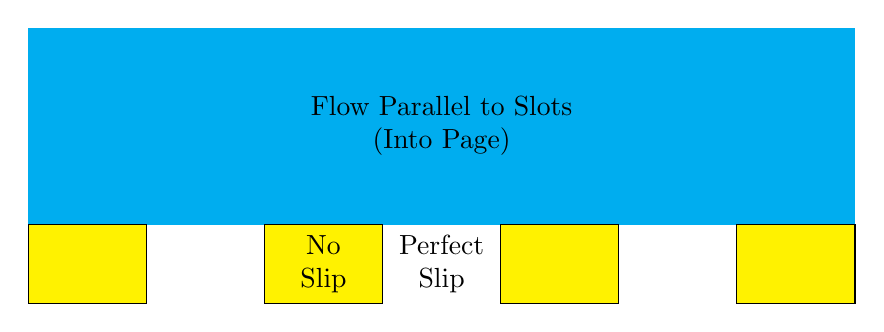
\begin{tikzpicture}

\coordinate (slotwidth) at +(1.5,0);
\coordinate (topright) at ($7*(slotwidth) + (0,2.5)$);
\fill[cyan] (0,0) rectangle (topright);

\path (slotwidth) ++(0,-1) coordinate (box);

\foreach \n in {0,1,2,3}
    \draw[fill=yellow] ($2*\n*(slotwidth)$) rectangle +(box);

\path ($2*(slotwidth) $) -- node[align=center] {No\\ Slip} +(box);
\path ($3*(slotwidth) $) -- node[align=center] {Perfect\\ Slip} +(box);

\path (0,0) -- node[align=center] {Flow Parallel to Slots\\ (Into Page)} (topright);

\end{tikzpicture}
\end{center}


\sep

It wasn't until 2003 that the case for flow \emph{transverse} to the slots was solved.  
In an article in the Journal of Fluid Mechanics that year \cite{LaugaStone2003}, Lauga and Stone study pressure-driven Stokes flow down a straight circular pipe.  They note that there is no analytic solution for the transverse case.  They derive dual series of equations, one for each boundary slip, which are simultaneously true.  They solve these numerically.  With $\phislip$ fixed, the asymptotic limit of the numerical solutions as period $L \rightarrow 0$ is the far field flow, implying an effective slip length:

\[ \beff= \frac{1}{2} \frac{L}{\pi}	\ln \sec \frac{\pi}{2} \phislip \]

which is exactly half the solution for parallel slots.

They provide a physical interpretation for the factor of two: An elongated body falling under its own weight falls twice as fast if it is oriented vertically than if it is oriented horizontally.

\begin{center}
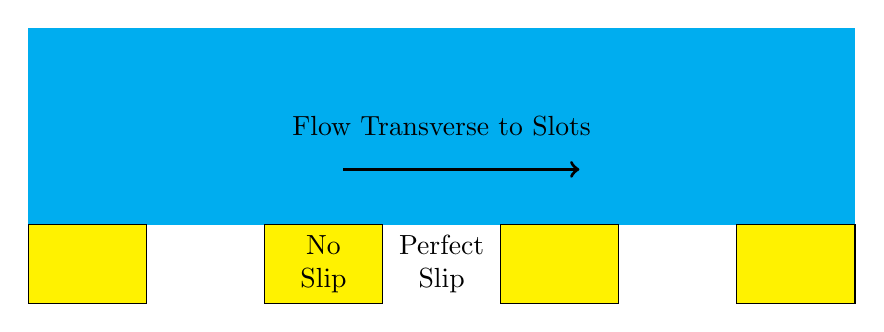
\begin{tikzpicture}

\coordinate (slotwidth) at +(1.5,0);
\coordinate (topright) at ($7*(slotwidth) + (0,2.5)$);
\fill[cyan] (0,0) rectangle (topright);

\path (slotwidth) ++(0,-1) coordinate (box);

\foreach \n in {0,1,2,3}
    \draw[fill=yellow] ($2*\n*(slotwidth)$) rectangle +(box);

\path ($2*(slotwidth) $) -- node[align=center] {No\\ Slip} +(box);
\path ($3*(slotwidth) $) -- node[align=center] {Perfect\\ Slip} +(box);

\path (0,0) -- node[align=center] {Flow Transverse to Slots} (topright);
\draw[->,very thick] (4,0.7) -- +(3,0);

\end{tikzpicture}
\end{center}


\subsection*{Flat No-Slip and Curved Perfect-Slip Parallel Strips}

Philip's foundational solution had flat strips of perfect slip.  Since these model a stress-free liquid-gas interface, it is reasonable to extend the model so that the perfect slip surface forms a slightly curved meniscus.  In 2007, Sbragaglia and Prosperetti did exactly that \cite{SbragagliaProsperetti2007}.  Using a dual-series technique, (rather than conformal mapping), they replicate Philip's result, and add a perturbation due the the curved meniscus.  They use as a small perturbation parameter:

\[ \epsilon = \frac{1}{2\pi} \frac{L}{2R} \]

where $R$ is the radius of curvature, and $L$ is the period of the pattern.  In the far field, the effective slip length is:

\[ \beff= \frac{L}{\pi}	\ln \sec \frac{\pi}{2} \phislip - \frac{L^2}{4R}\phislip^3 \int_0^1 
\frac{[1-\cos(\pi\phislip s)] (1-s^2) }{\cos(\pi\phislip s) - \cos(\pi\phislip)}
\; ds \]

They note that deformation of the meniscus \emph{reduces} the slip length. ``The physical origin of this phenomenon is due to the fact that, when the interface bows into the groove, the condition of free shear (perfect slip) is moved below the level $z=0$ of the undisturbed surface so that, on $z=0$, there is a residual nonzero stress."

\begin{center}
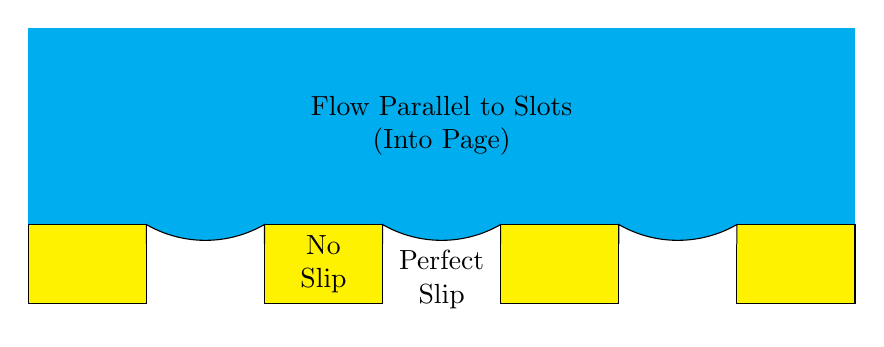
\begin{tikzpicture}

\coordinate (slotwidth) at +(1.5,0);
\coordinate (topright) at ($7*(slotwidth) + (0,2.5)$);
\fill[cyan] (0,-0.23) rectangle (topright);

\path (slotwidth) ++(0,-1) coordinate (box);

\foreach \n in {0,1,2,3}
    \draw[fill=yellow] ($2*\n*(slotwidth)$) rectangle +(box);

\path ($2*(slotwidth) $) -- node[align=center] {No\\ Slip} +(box);
\path ($3*(slotwidth) + (0,-0.2)$) -- node[align=center] {Perfect\\ Slip} +(box);

\path (0,0) -- node[align=center] {Flow Parallel to Slots\\ (Into Page)} (topright);

%\foreach \n in {1,3,5}
%    \draw[fill=cyan] ($\n*(slotwidth)$) arc (240:300:1.5);
    
\foreach \n in {1,3,5}
\draw[fill=white] ($\n*(slotwidth) + (0,-0.25) $) -- ++(0,0.25) arc (240:300:1.5) -- +(0,-0.25);

\end{tikzpicture}
\end{center}

\sep

Another variation is that the perfect-slip strips model a bubble type geometry, with the surface bulging up into the liquid.  In a 2009 paper in Physics of Fluids, Davis and Lauga consider this scenario \cite{DavisLauga2009a}.  Their model is still 2-dimensional Stokes flow, so that the `bubbles' can be considered to be the cross sections of spherical caps on top of channels full of air. Flow is thus transverse to the grating.  The channels have width $2c$, and the greater the air pressure therein, the further the bubble cap protrudes into the liquid.  The magnitude of protrusion is quantified by the angle $\theta$ that the bubble wall makes to the solid surface.

In the dilute limit, i.e. bubbles sparsely distributed on the surface, the effective slip tends to:

\begin{multline*}
\beff = c\pi \phislip \; \times \\
\int_0^{\infty}
\frac{s}{\sinh 2s(\pi -  \theta) + s \sin 2\theta}  \left[ \cos 2\theta + 
\frac{s \sin 2\theta \cosh s \pi + \sinh s(\pi - 2 \theta)}{\sinh s \pi}
\right] \; ds
\end{multline*}

\vspace{1em}

\begin{center}
\begin{tikzpicture}

\coordinate (width) at (10.5,0);
\fill[cyan] (0,2.5) rectangle (width);

\coordinate (b1) at (1.5,0);
\draw[fill=white] ($(b1) + (0,-1.5)$) -- ++(0,1.5) arc (145:35:1.07) -- +(0,-1.5) coordinate (p1);
\path (b1) -- node[above, align=center] {Perfect\\Slip} (p1);

\coordinate (b2) at (8,0);
\draw[fill=white] ($(b2) + (0,-1.5)$) -- ++(0,1.5) arc (145:35:1.07) -- +(0,-1.5) coordinate (p2);
\draw[<->] (b2) ++(0,-1) -- node[above] {$2c$} ($(p2) +(0,0.5)$);
\draw[dashed] (b2) -- +(0.8,0) (b2) -- +(55:1 cm);
\path (b2) ++(0.4,0.15) node {$\theta$};


\draw[fill=yellow] (0,0) ++(0,-1.5) rectangle (b1);
\draw[fill=yellow] (p1) rectangle (b2);
\draw[fill=yellow] (p2) rectangle (width);

\node at (5,0) [below] {No Slip};

\path (0,0) -- node[align=center] {Flow Transverse to Slots} (topright);
\draw[->,very thick] (4,0.7) -- +(3,0);

\end{tikzpicture}
\end{center}

They evaluate for various values of $\theta$, nondimensionalized by channel width.  They find good agreement with the numerical results of Steinberger \emph{et al} \cite{Steinberger2007} and Hyv\"{a}luoma and Harting \cite{HyvaluomaHarting2008}.

``The main features of the full numerical results are seen to be reproduced by our analytical model.  There exists a critical protrusion angle $ \theta_c$ above which the effect of the wall-attached bubbles displays a transition from reduced ($ \theta < \theta_c $) to enhanced friction ($ \theta > \theta_c $).  Our model predicts $ \theta \approx 65^{\circ} $, in good agreement with the results of [Steinberger \emph{et al}] ($ \theta \approx 62^{\circ} $) and [Hyv\"{a}luoma and Harting] ($ \theta \approx 69^{\circ} $). ''

\subsection*{Flat Surface, with Slip Length $\gg$ Period, Otherwise Arbitrary}


In 2007, we published in Phys. Rev. E \cite{HendyLund2007} a perturbative proof that --- to first order --- the effective slip length is the harmonic mean of the intrinsic slip lengths

\begin{equation*}
\beff = \left< \frac{1}{b} \right>^{-1}
\end{equation*}

This result is valid for a flat surface with an intrinsic slip length varying in one dimension over some period $L$.  The minimum slip length must be greater than the period $L$, but may otherwise be arbitrary.

\vspace{1em}
\colorbox[gray]{0.8}{ \textsc{3-D Flow} }
\vspace{0.5em} \\
In 2008, we published in ANZIAM Journal \cite{LundHendy2008} an extension of the above result for 3-dimensional flow over a flat surface with a square-periodic variation in intrinsic slip length.  The perturbative proof still required that $b_{\mathrm{minimum}} \gg L$, with $b$ otherwise arbitrary, and the result was the same harmonic mean formula:

\begin{equation*}
\beff = \left< \frac{1}{b} \right>^{-1}
\end{equation*}

This published result subsumes our published result from the previous year.  It is is fully presented in Chapter 5.

\subsection*{Rough Surface, with Slip Length $\gg$ Period, Otherwise Arbitrary}

Using a completely different technique --- homogenization --- we have proved that
for flow over a \emph{rough} surface with a slip length varying with the same period $L$ as the roughness, with the minimum slip length much greater than $L$,

\begin{equation*}
\beff = \left< \frac{\sqrt{1 + s^2}}{b} \right>^{-1}
\end{equation*}

This is the harmonic mean weighted by \emph{area of contact} --- not just footprint area.  ($s$ is the slope and $\sqrt{1+s^2}$ is the arc length.)  For a flat surface, this reduces to our previous perturbative result.

This proof was published in Phys. Rev. E in 2012 \cite{Lund2012}.  It is the centrepiece of this thesis, and is presented fully in Chapter 4.


\subsection*{Rough Surface of Single Intrinsic Slip}

Finally, there is an interesting relatively early result for a \emph{rough} surface with a \emph{single} unchanging intrinsic slip length.  In 1990 Einzel, Panzer and Liu \cite{EinzelPanzerLiu1990} studied a `weakly varying surface' of the form

\begin{equation*}
y(x) = \sum_n \left[ h_n^{\cos} \cos(nkx) + h_n^{\sin} \sin(nkx) \right]
\end{equation*} 

This Fourier surface has a \textbf{single} intrinsic slip length $b_0$.  In the `stick' limit, $kb_0 \ll 1$, the effective slip length is:

\begin{equation*}
\beff = b_0 - \sum_n nk \left[ (h_n^{\cos})^2 + (h_n^{\sin})^2  \right]
\end{equation*}

More interestingly, in the limit of perfect slip, $kb_0 \gg 1$, they get

\begin{equation*}
\beff = \left[ \frac{1}{b_0} + \sum_n (nk)^3 \left[ (h_n^{\cos})^2 + (h_n^{\sin})^2 \right]
 \right]^{-1}
\end{equation*}

They get a very similar result for incommensurate sine waves, so the result holds for pseudo-random roughness.

The interesting point is that even if a rough surface has \emph{perfect slip} i.e. infinite slip length, the effective slip length is still finite, because of the roughness.


\section*{Simplified Models, Scaling Laws and Numerics}

\subsection*{Models with Simplifying Assumptions}

In 2004, Tretheway and Meinhart \cite{TrethewayMeinhart2004} consider a variation of the binary surface wherein the gas-liquid interface has some large finite slip length, rather than an infinite slip length.  Piecing together the paper and an Erratum \cite{TrethewayMeinhartErratum2004} published 2 years later, it seems they claim that the intrinsic slip length for water of thickness $2D$ flowing over a rarefied gas layer of thickness $\delta$ is:

\begin{equation*}
b_{\mathrm{slip}} = \frac{1}{2D} \left( \frac{\mu_{water}}{\mu_{air}} \right)
\left[ 2D\delta + \delta^2 + \epsilon(4D + 2\delta) \right]
\end{equation*}

where $\epsilon$ is the slip length of the rarefied gas slipping over the solid.  $b_{\mathrm{slip}}$ is derived from a velocity equation $u_{\mathrm{slip}}$.  They combine this with the standard no-slip velocity equation (Couette flow):
``We combine the slip and no-slip [velocity] equations in a weighted average and calculate the cumulative velocity, $u_{\mathrm{cu.}}$, by

\begin{equation*}
u_{\mathrm{cu.}} = \phi u_{\mathrm{slip}} + (1-\phi) u_{\mathrm{no-slip}}
\end{equation*}

where $\phi$ is the fraction covered by gas. ..., we set the cumulative velocity at the air-water interface equal to the slip length times the shear rate at the air-water interface to obtain an equation for slip length ..."

\begin{equation*}
b_{\mathrm{cu.}} = \phi \frac{1}{2D} \left( \frac{\mu_{water}}{\mu_{air}} \right)
 \left[ 2D\delta + \delta^2 + \epsilon(4D + 2\delta) \right]
\end{equation*}

And that is the end of their analysis.  However, the observant reader may notice that

\begin{equation*}
b_{\mathrm{cu.}} = \phi b_{\mathrm{slip}} 
\end{equation*}

Perhaps due to the inconsistent notation of a derivation spread over a paper and an erratum published two years later, Tretheway and Meinhart do not mention this.

Furthermore, a careful reading seems to reveal that 
$ \partial_z u_{\mathrm{slip}} = \partial_z u_{\mathrm{no-slip}} = \dot{\gamma} $
If the shear rate does not depend on the local slip length, we can think about a binary surface with more general slip conditions --- not just `no slip', with local slip lengths defined via
$u_{\mathrm{slip}} = b_{\mathrm{slip}} \dot{\gamma}$ and $u_{\mathrm{low-slip}} = b_{\mathrm{low-slip}} \dot{\gamma}$.

Then for velocities at the $z=0$ boundary:
\begin{align*}
u_{\mathrm{cu.}} & = b_{\mathrm{cu.}} \partial_z u_{\mathrm{cu.}} \\
u_{\mathrm{cu.}} & = b_{\mathrm{cu.}} \partial_z
[ \phi u_{\mathrm{slip}} + (1-\phi) u_{\mathrm{low-slip}} ] \\
u_{\mathrm{cu.}} & = b_{\mathrm{cu.}} 
[ \phi \partial_z u_{\mathrm{slip}} + (1-\phi) \partial_z u_{\mathrm{low-slip}} ] \\
u_{\mathrm{cu.}} & = b_{\mathrm{cu.}} [ \phi \dot{\gamma} + (1-\phi) \dot{\gamma} ]\\
u_{\mathrm{cu.}} & = b_{\mathrm{cu.}} \dot{\gamma}\\
\phi u_{\mathrm{slip}} + (1-\phi) u_{\mathrm{low-slip}} & = b_{\mathrm{cu.}} \dot{\gamma} \\
\phi \frac{u_{\mathrm{slip}}}{\dot{\gamma}} + (1-\phi) \frac{ u_{\mathrm{low-slip}}} {\dot{\gamma}} & = b_{\mathrm{cu.}} \\
\phi b_{\mathrm{slip}} + (1-\phi) b_{\mathrm{low-slip}} & = b_{\mathrm{cu.}} \\
\left< b \right> & = b_{\mathrm{cu.}}
\end{align*}

Thus, their definition of `cumulative velocity' appears to imply that $b_{\mathrm{cu.}}$ is simply the area-weighted average of local slip lengths.  If $b_{\mathrm{low-slip}} = 0$, it follows that 
$ b_{\mathrm{cu.}} = \phi b_{\mathrm{slip}} $.

\sep

A rather more convincing assumption was used in a landmark article in Eur. Phys. Journal E in 2004 by Cecile Cottin-Bizonne \emph{et al} \cite{Cottin-Bizonne2004}.

Cottin-Bizonne and colleagues presented molecular dynamics fluid simulations, in which they observed the `dewetting transition', wherein the liquid sits on top of posts, giving a large effective slip length.  They do some numerical calculations to predict the effective slip length in various regimes.  

For the regime of \textbf{No-slip/Perfect-slip} strips, they find excellent agreement with the analytic results of J.\ R.\ Philip \cite{Philip1972} and Lauga and Stone \cite{LaugaStone2003}.  Now confident in their technique, they investigate other regimes.

For strips of \textbf{No-slip and Partial-slip} material, they find that $\beff$ is fixed by the smaller of the two lengths, $b_{\mathrm{slip}}$ and the period $L$.

$\bullet$ For low slip ($b_{\mathrm{slip}} < L$), $\beff$ increases linearly, roughly $\beff = b_{\mathrm{slip}} / 4$

$\bullet$ For high slip ( $b_{\mathrm{slip}} > 10L$), $\beff$ asymptotes to a fraction of $L$. Roughly $L/10$ for flow parallel to stripes, and $L/20$ for transverse flow.

\vspace{1em}

For stripes of \textbf{Partial-slip and Perfect-slip} material, they find that $\beff$ is determined by the \emph{larger} of $b_{\mathrm{slip}}$ and period $L$.

$\bullet$ For small slip ($b_{\mathrm{slip}} \ll L$), $\beff$ is fixed by the period $L$.

$\bullet$ For high slip ($b_{\mathrm{slip}} > L$), $\beff$ increases linearly with intrinsic slip.

They advance a `simple phenomenological model' to explain this linearity:

``We introduce the interfacial friction coefficient $\lambda$, defined by ... the continuity of the tangential stress $\sigma_s$ at the solid-liquid interface:
\begin{equation*}
\sigma_s = \eta \frac{\partial V}{\partial z} = \lambda V_s
\end{equation*}
where $\eta$ is the viscosity of the liquid and $V_s$ [is the slip velocity]. The interfacial friction coefficient $\lambda$ is then related to the slip length $b$ by
\begin{equation*}
\lambda = \frac{\eta}{b}
\end{equation*}
The effective friction coefficient $\Lambda = \frac{\eta}{\beff}$ can be interpreted as the \emph{averaged friction} over the different stripes, and we obtain, accordingly, the following result for the effective macroscopic slip length as a function of the microscopic ones:
\begin{equation*}
\beff = \left[ \phi \frac{1}{ b_{\mathrm{high}} }  + (1 -\phi) \frac{1}{ b_{\mathrm{low}}} \right]^{-1}
\end{equation*}
which is similar to the addition rule for resistors in parallel.

In the case $b_{\mathrm{high}} \rightarrow \infty$, we expect
\begin{equation*}
\beff = \frac{b_{\mathrm{low}}}{1-\phi} \;"
\end{equation*}

Cecile notes ``It is important to emphasize that its validity is limited to the case where both the slip lengths, $\bhigh$ and $\blow$, are larger than the roughness periodicity $L$. Note, however, that in practice, this relationship is valid down to $\blow > 0.1L$."

To the best of our knowledge, this is the first assertion that $\beff$ is the harmonic mean of intrinsic slip lengths.  This result inspired this thesis, which provides a rigorous derivation and extension of this harmonic mean formula.

\sep

In 2009, Ng and Wang \cite{NgWang2009} considered flow over the familiar binary surface of flat perfect-slip/partial-slip regions, with one difference: the perfect-slip gas-liquid interface was allowed to be some distance $d$ below the solid surface.  They did numerical evaluations of flow both parallel and transverse to the resulting `step function profile' surface.

They compare their numerics with the continuum modeling results of Cottin-Bizonne \emph{et al.}\ 2004 \cite{Cottin-Bizonne2004}, and find essentially perfect agreement.

However, their most interesting observation relates to the conventional completely flat binary surface.  They recall Cottin-Bizonne's proposal for $\beff$ for flow parallel to the strips:

\begin{equation*}
\beff = \frac{b_{\mathrm{solid}}}{1 - \phi}
\end{equation*}

which works very well for large $b_{\mathrm{solid}}$.  Ng and Wang have discovered that this is much improved by simply gluing on J.\ Philip's exact result \cite{Philip1972} for $b_{\mathrm{solid}}=0$:

\begin{equation*}
\beff =  \frac{L}{\pi} \ln \left[ \sec \left( \frac{\pi}{2} \phi \right) \right] +
 \frac{b_{\mathrm{solid}}}{1 - \phi}
\end{equation*}

And similarly, for transverse flow, glue on the exact solution of Lauga and Stone \cite{LaugaStone2003}
\begin{equation*}
\beff = \frac{1}{2}  \frac{L}{\pi} \ln \left[ \sec \left( \frac{\pi}{2} \phi \right) \right] +
 \frac{b_{\mathrm{solid}}}{1 - \phi}
\end{equation*}

Ng and Wang test these extended formulae numerically, and find that they give a maximum error of 3\% -- 6\%, compared with Cottin-Bizonne's original formula which can have a maximum error of more than 50\% for small $b_{\mathrm{solid}}$.


\subsection*{The Scaling Laws of Ybert \emph{et al}}

Possibly the highest-profile article relating to effective slip length is the 2007 article in Physics of Fluids by Ybert and coworkers, entitled ``Achieving large slip with superhydrophobic surfaces: Scaling laws for generic geometries" \cite{Ybert2007}. The authors form a research group at Lyon, France, which includes Cecile Cottin-Bizonne.  Hence, the paper makes the same assumptions as the `phenomenological model' of Cottin-Bizonne 2004 \cite{Cottin-Bizonne2004}, and takes them in a slightly different direction, to get scaling laws for various geometries.
The paper is sufficiently influential, and the derivation sufficiently elegant, that we essentially reproduce it here.


At the heart of the model is the concept of stress balance.  Consider the stress on a plane of infinitesimal area located on the fluid boundary.

\begin{center}
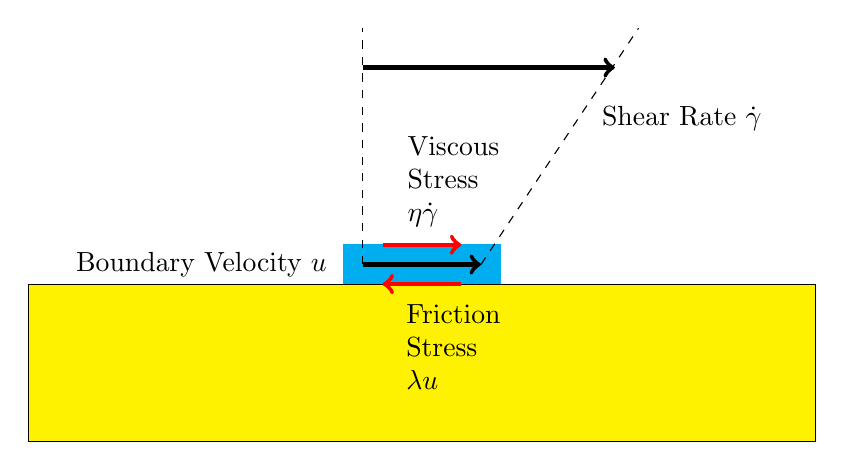
\begin{tikzpicture}

\filldraw[color=cyan] (0,0) rectangle (2,0.5);
\draw [fill=yellow] (-4,0) rectangle (6,-2);

\coordinate (ref) at (0.25,0.25);
\draw[->,ultra thick] (ref) -- ++(1.5,0);
\draw[dashed] (ref) -- ++(0,3);
\draw[->, ultra thick] (ref) ++(0,2.5) -- ++(3.2,0);
\draw[dashed] (ref) ++(1.5,0) -- ++(2,3);

\node at (-1.8,0.25) {Boundary Velocity $u$};
\node at (4.3,2.1) {Shear Rate $\dot{\gamma}$};

%%%%%%%%%%%%%%  Stress arrows
\draw [<-, ultra thick, color=red] (0.5,0) -- ++(1,0);
\draw [->, ultra thick, color=red] (0.5,0.5) -- ++(1,0);

\node at (1.4,1.3) [align=left] {Viscous\\ Stress\\ $\eta \dot{\gamma} $};
\node at (1.4,-0.8) [align=left] {Friction\\Stress\\ $\lambda u$};

\end{tikzpicture}
\end{center}

At equilibrium, the stresses balance:

\begin{equation*}
\sigma = \eta \dot{\gamma} = \lambda u
\end{equation*}

The stress can be \emph{averaged} over the entire surface (or over one period):

\begin{equation*}
\left< \sigma \right> = \left< \eta \dot{\gamma} \right> = \left< \lambda u \right>
\end{equation*}

Now the viscosity $\eta$ can be considered constant throughout the fluid, so that $  \left< \eta \dot{\gamma} \right> = \eta \left< \dot{\gamma} \right> $.  But the friction coefficient $\lambda$ is not constant.  Therefore, Ybert \emph{et al} define an effective friction coefficient such that:

\begin{equation*}
\left< \lambda u \right> = \lambda_{\mathrm{eff}} \left< u \right>
\end{equation*}
\begin{equation*}
\text{But then of course} \quad
\eta \left< \dot{\gamma} \right> = \lambda_{\mathrm{eff}} \left< u \right>
%\end{equation*}
\quad \text{rearranges to}  \quad
%\begin{equation*}
\left< u \right> = \frac{\eta}{ \lambda_{\mathrm{eff}} } \left< \dot{\gamma} \right> 
\end{equation*}
which defines some kind of effective slip length:
\begin{equation*}
\beff = \frac{\eta}{ \lambda_{\mathrm{eff}} }  
\end{equation*}

This definition of $\beff$ relates the \emph{area average} boundary velocity to the \emph{area average} of the shear rate at the boundary.

\begin{equation*}
\left< u \right> = \beff \left< \dot{\gamma} \right> 
\end{equation*}

\vspace*{1em}
\colorbox[gray]{0.8}{ \textsc{2-D Flow over Perfect-slip/No-slip Surface} }
\vspace{0.5em}

The average stress on a binary surface can be decomposed into the area-weighted averages of the `subaverages' of stress over the liquid-gas interface and the liquid-solid interface:

Then 
\begin{equation*}
\left< \sigma \right> = \phi \left< \sigma_{\mathrm{gas}} \right> + 
\phisol \left<  \sigsol \right> 
\end{equation*}

If the gas-liquid interface is considered to be perfect-slip or \emph{no-shear}, there is no stress; $ \sigma_{\mathrm{gas}} = 0 $.  Hence 
\begin{equation*}
\left< \sigma \right> = \phisol \left<  \sigsol \right>
\end{equation*}

\begin{equation*}
\text{Viscosity $\eta$ is constant, so} \;\;\;
\left< \sigsol \right> = \eta \left< \dot{\gamma}_{\mathrm{solid}} \right>
\end{equation*}
\begin{equation*}
\text{For flow over a flat surface, `simple shear' obtains:} \quad
\dot{\gamma}_{\mathrm{solid}} = \frac{\partial u}{\partial z}
\end{equation*}

So
\begin{equation*}
\left< \sigsol \right> = \eta \left< \frac{\partial u}{\partial z} \right>
\end{equation*}

\vspace{1em}
\colorbox[gray]{0.8}{ \textsc{Case where $\phisol \rightarrow 0$, Mostly Plug-like flow.} }
\vspace{0.5em}

\begin{center}
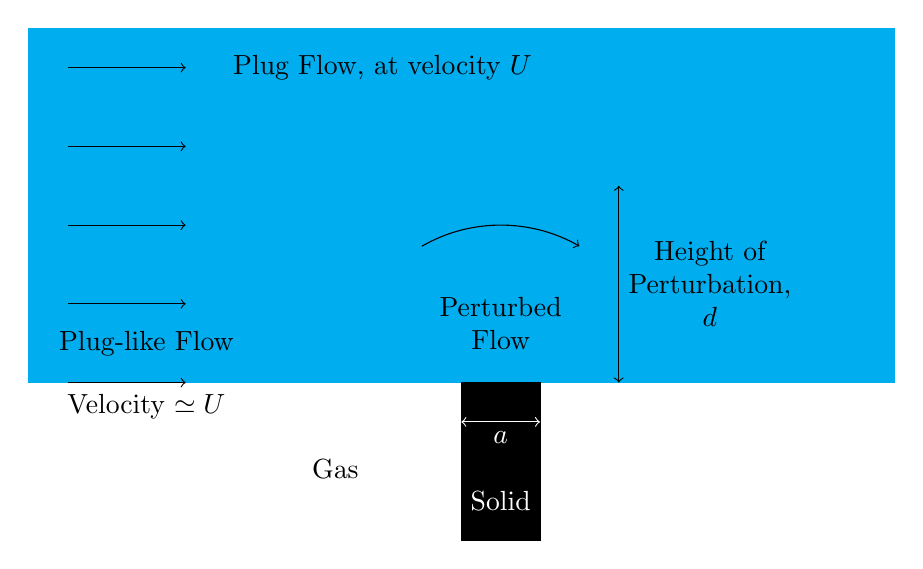
\begin{tikzpicture}

\filldraw[color=cyan] (-5.5,0) rectangle (5.5,4.5);
\filldraw (0,0) rectangle (1,-2);

\node at (-1.6,-1.1) {Gas};

\draw[<->,color=white] (0,-0.5) -- node [below] {$a$} ++(1,0);
\node at (0.5,-1.5) [color=white] {Solid};

\node at (0.5,0.75) [align=center] {Perturbed\\Flow};
\draw[<->] (2,0) -- node[right,align=center] {Height of \\Perturbation,\\ $d$} ++(0,2.5);

\draw (0.5,2) arc (90:120:2cm);
\draw[->] (0.5,2) arc (90:60: 2cm);

\foreach \z in {0,1,2,3,4}
     { \draw[->] (-5,\z) -- ++(1.5,0);
      % \draw[->] (4,\z) -- ++(1,0);
      }
       
\node at (-4,0.5) {Plug-like Flow};
\node at (-4,-0.3) {Velocity $\simeq U$};
%\node at (4,0.5)  {Plug-like Flow};
\node at (-1,4) {Plug Flow, at velocity $U$};
       
\end{tikzpicture}
\end{center}

The flow is mostly plug-like, with some characteristic velocity $U$.  The only place it is not plug-like is in the vicinity of the post.  The fluid sticks to the top of the post (no-slip), perturbing the plug-like flow.  The perturbed region extends some (arbitrary) distance $d$ above the post, at which point the velocity is (arbitrarily) close to $U$ again.  

\begin{center}
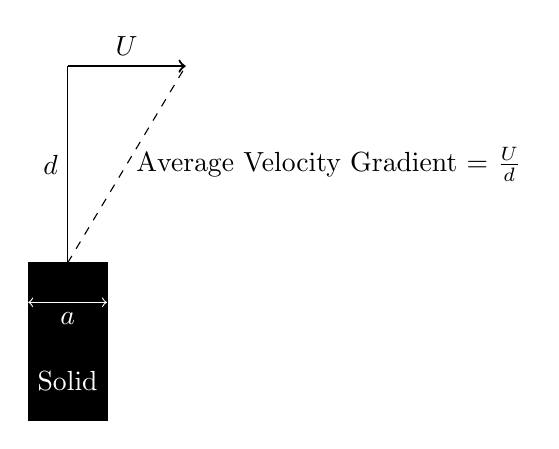
\begin{tikzpicture}

\filldraw (-0.5,0) rectangle ++(1,-2);
\draw[<->,color=white] (-0.5,-0.5) -- node [below] {$a$} ++(1,0);
\node at (0,-1.5) [color=white] {Solid};

\draw (0,0) -- node [left] {$d$} +(0,2.5);
\draw [->,thick] (0,2.5) -- node[above] {$U$} +(1.5,0);
\draw [dashed] (0,0) -- node[right] {Average Velocity Gradient = $\frac{U}{d}$} (1.5,2.5);

\end{tikzpicture}
\end{center}

Thus, the velocity changes from 0 to $U$ in distance $d$; the average velocity gradient is therefore
\begin{equation*}
\left< \frac{\partial u}{\partial z} \right> = \frac{U}{d}
\end{equation*}

Now, $d$ scales as $a$.  This is shown by dimensional analysis using the Buckingham Pi theorem in Appendix D.

Hence,
\begin{equation*}
\left< \frac{\partial u}{\partial z} \right> \sim \frac{U}{a}
\end{equation*}

Ybert and company justify the foregoing succintly: ``To estimate $ \left< \gamsol \right> $, we recall that the Stokes equation has a Laplacian form, which strongly couples the spatial dependence of the velocity profile along the different axes ($x,y,z$). This implies that $ \left< \gamsol \right> = \left< \partial u / \partial z \right> \sim U/a $, with $a$ the typical size of the solid area."

Thus, 
\begin{equation*}
\left< \sigsol \right> \sim \eta \frac{U}{a}
\end{equation*}
and
\begin{equation*}
\left< \sigma \right> \sim \phisol \eta \frac{U}{a}
\end{equation*}

The other interesting thing about mostly plug-like flow is that most of the fluid at the boundary is moving at the characteristic velocity $U$. So
\begin{equation*}
\left< u \right> \simeq U
\end{equation*}

Thus we have
\begin{equation*}
\eta \left< \dot{\gamma} \right> = \left< \sigma \right> \sim
  \frac{ \phisol \eta} {a} \left< u \right>
\end{equation*}
simplifying to:
\begin{equation*}
\left< u \right> \sim \frac{a}{\phisol}  \left< \dot{\gamma} \right>
\end{equation*}


defining
\begin{equation*}
\beff \sim  \frac{a}{\phisol} 
\end{equation*}

Thus in the limit of small solid fraction $\phisol$, Ybert \emph{et al} have shown that
\begin{equation*}
\beff \sim \alpha  \frac{a}{\phisol} 
\end{equation*}
where $\alpha$ is a prefactor that depends on the geometry of the surface.  This is the main result of Ybert \emph{et al} 2007 \cite{Ybert2007}.


\vspace{1em}
\colorbox[gray]{0.8}{ \textsc{Other Results} }
\vspace{0.5em}


Ybert \emph{et al} compare this scaling law with the exact result of J.\ R.\ Philip \cite{Philip1972}.  For the striped surface in question, $\phisol = a/L$, so the scaling law is:
\begin{equation*}
\beff \sim L
\end{equation*}
They note that in the limit of small $\phisol$, Philip's exact solution is similar, having only logarithmic dependence on $\phisol$: $\beff \sim L \log \phisol $


\vspace{1em}

If the surface is a forest of nanopillars, $\phisol = (a/L)^2$, so the scaling law is:
\begin{equation*}
\beff \sim  \frac{a}{\sqrt{ \phisol}} 
\end{equation*}

\vspace{1em}
Finally, if the no-slip condition is relaxed and some finite slip length $b_s$ holds on the solid post, the scaling law is modified to:
\begin{equation*}
\beff \sim  \frac{a + b_s}{\phisol} 
\end{equation*}

\vspace{1em}
For completeness, they consider the case of vanishing gas area.  Flow over a surface with very narrow gas gaps of width $l$ will be close to Couette flow, with:
\begin{equation*}
\beff \sim l (1-\phisol) 
\end{equation*}

The paper also features a few more formulae of a more speculative nature, which we won't mention here.

\subsection*{Numerics}

As already mentioned, Ng and Wang in 2009 \cite{NgWang2009} did numerical studies of flow over a grating, in both parallel and transverse orientations. They derive eigenfunction expansions of the flow solutions, which are solved numerically.  The effective slip lengths extracted have essentially perfect agreement with the continuum modeling of Cottin-Bizonne 2004 \cite{Cottin-Bizonne2004}.

\sep

In their second paper of 2009 \cite{DavisLauga2009b}, Davis and Lauga consider Stokes flow over a mesh of thin wires or strips, with large square air gaps in between.  The surface is considered to be flat, with no-slip on the strips, and perfect-slip on the liquid-air interface.  The period of the square-periodic mesh is $L$, and the width of the strips is $\epsilon L$.

\begin{center}
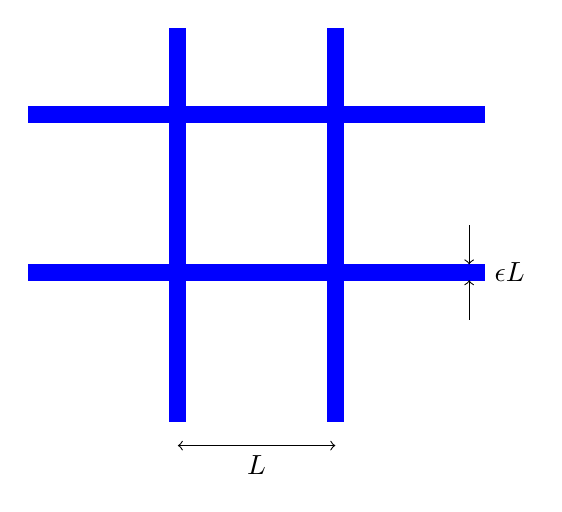
\begin{tikzpicture}

\filldraw[color=blue] (0,0) rectangle +(0.2,5);
\filldraw[color=blue] (2,0) rectangle +(0.2,5);
\draw[<->] (0.1,-0.3) -- node[below]{$L$} +(2,0);

\filldraw[color=blue] (-1.8,2) rectangle +(5.8,-0.2);
\filldraw[color=blue] (-1.8,4) rectangle +(5.8,-0.2);
\draw[<-] (3.8,2) -- +(0,0.5);
\draw[<-] (3.8,1.8) -- +(0,-0.5);
\node at (4,1.9)[right] {$\epsilon L$};

\end{tikzpicture}
\end{center}

Davis and Lauga use a method of superposition of singularities, and end up with an infinite system of linear equations.  Then $\beff = L/\pi (A_0 + B_0)$ where $A_0$ and $B_0$ are the zeroth-order coefficients of the system of equations.

They solve numerically for $A_0$ and $B_0$ by truncating the infinite system at $N$ equations.  (Truncating at $N=1000$ rather than $N=100$ changed the computed $\beff$ by less than $0.01\%$.) After computing $\beff$ for various values of $\epsilon$, they derive a least-squares fit formula:

\begin{equation*}
\beff = -0.107 L \ln \phisol + 0.003L
\end{equation*}

Finally, they offer `simple estimates' -- solutions from truncating the infinite series at $N=1$ and $N=2$ terms. For $N=1$:

\begin{equation*}
\beff = \frac{L}{3\pi} \ln \left( \frac{2}{\pi \epsilon} \right)
\end{equation*}

The simple estimate for $N=2$ is more complicated.  These simple estimates overestimate $\beff$ by up to 10\%, but converge on the correct result as $\epsilon \rightarrow 0$.

\subsection*{Coefficients Evaluated for Ybert's Scaling Laws}

The influential scaling law paper by Ybert \emph{et al} \cite{Ybert2007} inspired researchers to find the relevant coefficients by numerical or approximate methods.

In 2010, Ng and Wang \cite{NgWang2010} continued their approach of numerically solving eigenfunction expansions, to find the scaling coefficients.

For flow over superhydrophobic surfaces, with the solid posts occupying a small area fraction, Ybert had proposed:
\begin{equation*}
\beff \sim \frac{1}{\sqrt{\phisol}}
\end{equation*}
From their numerical data, Ng and Wang fit the parameters:

\begin{align*}
\beff &= \frac{0.34}{\sqrt{\phisol}} - 0.468 \quad \text{for circular posts,} \\
\beff &= \frac{0.33}{\sqrt{\phisol}} - 0.461 \quad \text{for square posts.}
\end{align*}

And so on and so on.  Ng and Wang present numerically fitted parameters for the nanobubble case ($\phisol \rightarrow 1$), for cases with finite slip on the solid, and for cases where the geometry is elliptical or rectangular rather than simply circular or square.

\sep

In 2010, Davis and Lauga \cite{DavisLauga2010} studied Stokes flow over a superhydrophobic surface comprising a rectangular array of circular posts, each of radius $a$.

\begin{center}
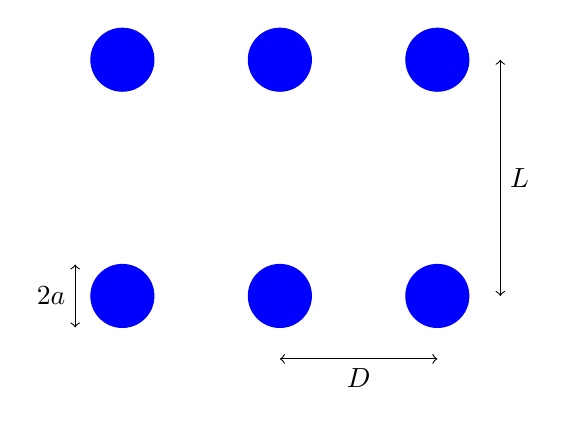
\begin{tikzpicture}

\filldraw[color=blue] (0,0) circle (4mm);
\filldraw[color=blue] (2,0) circle (4mm);
\filldraw[color=blue] (4,0) circle (4mm);
\filldraw[color=blue] (0,3) circle (4mm);
\filldraw[color=blue] (2,3) circle (4mm);
\filldraw[color=blue] (4,3) circle (4mm);

\draw[<->] (-0.6,-0.4) -- node[left]{$2a$} +(0,0.8);
\draw[<->] (2,-0.8) -- node[below]{$D$} +(2,0);
\draw[<->] (4.8,0) -- node[right]{$L$} +(0,3);

\end{tikzpicture}
\end{center}

As their point of departure, they take the scaling law proposed in Ybert \emph{et al} 2007 for the limit of small $\phisol$:
\begin{equation*}
\beff \sim \frac{A}{\sqrt{\phisol}} L - BL
\end{equation*}

They attack the problem with Fourier transform techniques, and end up with an infinite system of linear equations for coefficients.  They make an `asymptotic estimate' of the coefficients, and get:
\begin{equation*}
\beff \sim \frac{3}{16} \sqrt{ \frac{\pi}{\phisol}} \sqrt{DL}
\end{equation*}
If the array is square, this reduces to:
\begin{equation*}
\beff \sim \frac{3}{16} \sqrt{ \frac{\pi}{\phisol}} L
\end{equation*}
Adding the next-order correction term gives (for the square array):
\begin{equation*}
\beff \sim \frac{3}{16} \sqrt{ \frac{\pi}{\phisol}} L - \frac{3}{2\pi} \ln(1 + \sqrt{2})L
\end{equation*}
in the limit of low $\phisol$.

They compare their analytical asymptotic estimate with previous numerical work: ``The quantitative agreement between our model and previous numerical work is remarkable... we find that the error between our simple model, and numerics of Ng and Wang (2010) \cite{NgWang2010} is about 1.8\%, while the error between our model and the computations of Ybert \emph{et al} (2007) \cite{Ybert2007} is about 3.9\%."



\section*{Conclusion}

There exists only on the order of a dozen expressions for the effective slip length of a mixed-slip surface.  Only a handful of them are exact results that have been rigorously derived, including the seminal work of J.\ R.\ Philip in 1972 \cite{Philip1972}, the work of Lauga and Stone in 2003 \cite{LaugaStone2003}, and our own recent papers \cite{HendyLund2007,LundHendy2008,Lund2012}, which form the core of this thesis.

A simple phenomenological model was proposed by the Lyon group in the paper by Cottin-Bizonne \emph{et al} \cite{Cottin-Bizonne2004}, leading to the suggestion that
\begin{equation*}
\beff = \left<  \frac{1}{b} \right>^{-1}
\end{equation*}
This thesis proves this and extends it to the case of rough surfaces.  The same model inspired the derivation of several scaling laws, which appear in the highly influential paper of 2007 by Ybert \emph{et al} \cite{Ybert2007}.

The scaling laws have been refined by various researchers, by finding appropriate coefficients via numerical or approximate methods.

\begin{center} \vspace{3em} \Coffeecup \end{center}

\bibliography{Lund_Thesis.bib}
\bibliographystyle{plain}

\end{document}



